\documentclass[letterpaper,twocolumn,10pt]{article}
\usepackage{usenix}
\usepackage[boxed, ruled, noline, noend]{algorithm2e}
\usepackage[letterpaper,left=1in,right=1in,top=1in,bottom=1in]{geometry}
%\usepackage[small,compact]{titlesec}
\usepackage[font={small,bf}]{caption}    % added 9/10/13
\usepackage[nolineno,noindent,norules]{lgrind}
\usepackage{tightenum}
\usepackage{float}
\usepackage{xspace}
\usepackage{times,pifont}
\usepackage{mathptmx}
\usepackage{subfig,graphics,graphicx,color}
\usepackage{multirow}
\usepackage{dblfloatfix} %% correctly orders single- and double-col figures
\usepackage{hyphenat}
\usepackage{mathrsfs}
\usepackage{subfig}
\usepackage{amssymb,amsmath,centernot}
\usepackage{lastpage}
\usepackage{flushend}
\usepackage{hhline}
\usepackage{authblk}
\usepackage{pifont}
\usepackage{listings}
\usepackage[hyphens]{url}
%\newcommand{\doi}{XXXXXX}


%%% ================= START of SOSP '13 template ================= 
% \makeatletter
% 
% \def\ftype@copyrightbox{8}
% \def\@copyrightspace{
% \@float{copyrightbox}[b]
% \begin{center}
% \setlength{\unitlength}{1pc}
% \begin{picture}(20,6.0) 
% \put(0,3){\parbox{\columnwidth}{\scriptsize
% 
% %*** SAMPLE. AUTHOR PUT SUPPLIED TEXT HERE ****
% 
% \noindent
% \rule{6.0 cm}{0.2pt}\\
% Permissiondddd to make digital or hard copies of part or all of this work 
% for personal or classroom use is granted without fee provided that
% copies are not made or distributed for profit or commercial advantage 
% and that copies bear this notice and the full citation on the first
% page. Copyrights for third-party components of this work must be
% honored.  For all other uses, contact the Owner/Author. 
% 
% \vspace{\baselineskip}\noindent
% Copyright is held by the Owner/Author(s).\\
% \textit{SOSP'15}.\\
% ACM XXXXXXX.
% 
% \noindent
% http://dx.doi.org/\doi}
% }
% \end{picture}
% \end{center}
% \end@float}
% 
% \def\maketitle{\par
%  \begingroup
%    \def\thefootnote{\fnsymbol{footnote}}
%    \def\@makefnmark{\hbox
%        to 0pt{$^{\@thefnmark}$\hss}}
%      \twocolumn[\@maketitle]
% \@thanks
%  \endgroup
%  \setcounter{footnote}{0}
%  \let\maketitle\relax
%  \let\@maketitle\relax
%  \gdef\@thanks{}\gdef\@author{}\gdef\@title{}\gdef\@subtitle{}\let\thanks\relax
%  \@copyrightspace}
% 
% \makeatother

%%% ================= END of SOSP '13 template ================= 



%\newcommand{\comment}[1]{}
\frenchspacing

%\doublespacing

%%%%%%%%%%%%%%%%%%%%%%%%%%%%
%     macro

\newcommand{\xxx}[0]{\textsc{Falcon}\xspace}
\newcommand{\paxos}[0]{\textsc{Paxos}\xspace}
\newcommand{\mytitle}[0]{\textbf {Fast, General State Machine 
Replication via RDMA-accelerated \paxos}}
\newcommand{\mykeywords}[0]{State Machine Replication, Fault Tolerance, Stable 
and Deterministic Multithreading, Software Reliability}

%%%%%%%%%%%%%%%%%%%%%%%%%%%%%%%%%%%%%%%%%%%%%%%%%%%%%%%%%%%%%%%%%
% hyperref stuff

%\usepackage[square,comma,numbers,sort]{natbib}
\usepackage{hypernat}
\usepackage{hyperref}

%% fill in pdf info here
\hypersetup{%
colorlinks=false,
pdfborder={0 0 0},
pdftitle={\mytitle},
pdfkeywords={\mykeywords},
bookmarksnumbered,
pdfstartview={FitH},
urlcolor=cyan,
pdfpagelabels=true,
pdfdisplaydoctitle=true,
}%

%\usepackage{breakurl}
%\usepackage[all]{hypcap}
%\renewcommand{\url}{\burl}

%%%%%%%%%%%%%%%%%%%%%%%%%%%%%%%%%%%%%%%%%%%%%%%%%%%%%%%%%%%%
% Some NICE fonts

\newfont{\BIG}{cminch}                             %--- One-inch font
\newfont{\sfbHuge}{cmssbx10 scaled\magstep5}       %-- 25pt sans serif bold
\newfont{\sfbLarger}{cmssbx10 scaled\magstep3}   %-- 12+pt sans serif boldd
\newfont{\sfblarger}{cmssbx10 scaled\magstep2}   %-- 12+pt sans serif bold
\newfont{\sfblarge}{cmssbx10 scaled\magstep1}      %-- 12pt sans serif bold
\newfont{\sfbeleven}{cmssbx10 scaled\magstephalf}  %-- 11pt sans serif bold
\newfont{\sfb}{cmssbx10}                           %-- 10pt sans serif bold
\newfont{\sfeight}{cmss8}                          %-- 8pt sans serif

%%%%%%%%%%%%%%%%%%%%%%%%
%    space tweaking

%\textwidth = 6.5 in
%\textheight = 9.0 in
%\setlength{\topmargin}{-.5in}

%\headheight = 0.0 in
%\headsep = 0.0 in
%\parskip = 0.2in
%\parindent = 0.0in

\renewcommand{\topfraction}{0.95}
%\addtolength{\textfloatsep}{-0.1in}
%\addtolength{\floatsep}{0.025in}
\renewcommand\floatpagefraction{.9}
%\renewcommand\bottomfraction{.9}
\renewcommand\textfraction{.1}

\setlength{\parindent}{9pt}

% Rescue
\makeatletter
\def\v#1{{\mbox{\fontfamily{cmtt}\fontsize{\f@size}{\f@size}\selectfont #1}}}

\newcommand{\cmark}{\ding{51}}%
\newcommand{\xmark}{\ding{55}}%


\newcommand{\dmt}[0]{DMT\xspace}
\newcommand{\smt}[0]{StableMT\xspace}
\newcommand{\smr}[0]{SMR\xspace}

\newcommand{\tsan}[0]{\textsc{TSan}\xspace}
\newcommand{\valgrind}[0]{\textsc{Valgrind}\xspace}
\newcommand{\ski}[0]{\textsc{Ski}\xspace}
\newcommand{\racepro}[0]{\textsc{RacePro}\xspace}
\newcommand{\criu}[0]{\textsc{CRIU}\xspace}
\newcommand{\lxc}[0]{\textsc{LXC}\xspace}
\newcommand{\tern}[0]{\textsc{Tern}\xspace}
\newcommand{\peregrine}[0]{\textsc{Peregrine}\xspace}
\newcommand{\parrot}[0]{\textsc{Parrot}\xspace}
\newcommand{\repframe}[0]{\textsc{RepFrame}\xspace}
\newcommand{\grace}[0]{Grace\xspace}
\newcommand{\coredet}[0]{\textsc{CoreDet}\xspace}
\newcommand{\kendo}[0]{Kendo\xspace}
\newcommand{\dthreads}[0]{\textsc{DThreads}\xspace}
\newcommand{\determinator}[0]{Determinator\xspace}
\newcommand{\dos}[0]{dOS\xspace}
\newcommand{\ddos}[0]{DDOS\xspace}
\newcommand{\timealgo}[0]{time bubbling\xspace}
\newcommand{\ldpreload}[0]{LD\_PRELOAD\xspace}
\newcommand{\ntimeout}[0]{$W_{timeout}$\xspace}
\newcommand{\nclock}[0]{$N_{clock}$\xspace}
\newcommand{\us}[0]{\(\mu\text{s}\)\xspace}


\newcommand{\windows}{\v{Windows}\xspace}
\newcommand{\chrome}{\v{Chrome}\xspace}
\newcommand{\moonlight}{\v{Moonlight}\xspace}
\newcommand{\linux}{\v{Linux}\xspace}
\newcommand{\macos}{\v{Mac OS}\xspace}
\newcommand{\ios}{\v{iOS}\xspace}
\newcommand{\darwin}{\v{Darwin}\xspace}
\newcommand{\iexplorer}{\v{IE}\xspace}
\newcommand{\libsafe}{\v{Libsafe}\xspace}
\newcommand{\libvirt}{\v{Libvirt}\xspace}
\newcommand{\freebsd}{\v{FreeBSD}\xspace}
\newcommand{\kde}{\v{KDE}\xspace}
\newcommand{\ssdb}{\v{SSDB}\xspace}
\newcommand{\apache}{\v{Apache}\xspace}
\newcommand{\mysql}{\v{MySQL}\xspace}
\newcommand{\mongoose}[0]{\v{Mongoose}\xspace}
\newcommand{\ab}{\v{ApacheBench}\xspace}
\newcommand{\clamav}{\v{ClamAV}\xspace}
\newcommand{\upnp}{uPnP\xspace}
\newcommand{\mediatomb}{\v{MediaTomb}\xspace}
\newcommand{\memcached}{\v{Memcached}\xspace}
\newcommand{\mencoder}{\v{mencoder}\xspace}
\newcommand{\mongodb}{\v{MongoDB}\xspace}
\newcommand{\tftp}{\v{Open TFTP}\xspace}
\newcommand{\calvin}{\v{Calvin}\xspace}
% \newcommand{\ssdb}{\v{SSDB}\xspace}
\newcommand{\sysbench}{\v{SysBench}\xspace}
\newcommand{\zookeeper}{\v{ZooKeeper}\xspace}


\newcommand{\aget}[0]{\v{aget}\xspace}
\newcommand{\pthread}[0]{\mbox{Pthreads}\xspace}
\newcommand{\openldap}[0]{{OpenLDAP}\xspace}
\newcommand{\redis}[0]{{Redis}\xspace}
\newcommand{\bdb}[0]{{Berkeley DB}\xspace}
\newcommand{\vtune}[0]{\v{VTune}\xspace}
\newcommand{\http}[0]{\mbox{HTTP}\xspace}

% In short.
\newcommand{\eg}{{e.g.}}
\newcommand{\ie}{{i.e.}}
\newcommand{\etc}{{etc}}
\newcommand{\para}[1]{\vspace{.00in}\noindent{\bf #1}}
\newcommand{\wrt}{{w.r.t. }}
\newcommand{\cf}{{cf. }}

% Synch and network operations.
\newcommand{\checktimebubble}[0]{\v{check\_add\_timebubble()}\xspace}
\newcommand{\mutexlock}[0]{\v{pthread\_mutex\_lock()}\xspace}
\newcommand{\connect}[0]{\v{connect()}\xspace}
\newcommand{\send}[0]{\v{send()}\xspace}
\newcommand{\sendto}[0]{\v{sendto()}\xspace}
\newcommand{\sendmsg}[0]{\v{sendmsg()}\xspace}
\newcommand{\mywrite}[0]{\v{write()}\xspace}
\newcommand{\pwrite}[0]{\v{pwrite()}\xspace}
\newcommand{\close}[0]{\v{close()}\xspace}
\newcommand{\recv}[0]{\v{recv()}\xspace}
\newcommand{\recvfrom}[0]{\v{recvfrom()}\xspace}
\newcommand{\myread}[0]{\v{read()}\xspace}
\newcommand{\select}[0]{\v{select()}\xspace}
\newcommand{\poll}[0]{\v{poll()}\xspace}
\newcommand{\epollwait}[0]{\v{epoll\_wait()}\xspace}
\newcommand{\accept}[0]{\v{accept()}\xspace}
\newcommand{\uselib}[0]{\v{uselib()}\xspace}

% Parrot primitives.
\newcommand{\getturn}[0]{\v{get\_turn()}\xspace}
\newcommand{\putturn}[0]{\v{put\_turn()}\xspace}
\newcommand{\wait}[0]{\v{wait()}\xspace}
\newcommand{\signal}[0]{\v{signal()}\xspace}

% Evaluation stats.
\newcommand{\github}[0]{\url{github.com/osdi16-pXXX/falcon}}
\newcommand{\npopularprog}[0]{9\xspace}
\newcommand{\nprog}[0]{10\xspace}
\newcommand{\nkvprog}[0]{4\xspace}
\newcommand{\nsqlprog}[0]{2\xspace}
\newcommand{\tputoverhead}[0]{9.9\%\xspace} %TBD
\newcommand{\latencyoverhead}[0]{4.4\%\xspace} %TBD
\newcommand{\fasterthanzookeeper}[0]{8.9X\xspace}%TBD
\newcommand{\nlinescalvin}[0]{23\xspace}%TBD
% \newcommand{\fasterthanzookeeper}[0]{8.9X\xspace}%TBD

\def\LGfsize{\footnotesize}
%\pagestyle{empty}


% \conferenceinfo{SOSP'15}{October 4--7, 2015, Monterey, CA}
% \copyrightyear{2015} 
% \copyrightdata{978-1-4503-3834-9/15/10} 
% \doi{2815400.2815427}

\title{\mytitle}
% \authorinfo{XXX}{YYY}

\author[*]{Paper \#83}
% \author[*]{Heming Cui}
% \setlength{\affilsep}{0.5em}
% \renewcommand\AB@affilsepx{\hspace{28.0 mm}\protect\Affilfont}
% \affil[+]{\textrm\fontsize{10}{10}\selectfont The University of Hong Kong}
% \affil[*]{\textrm Columbia University}
% \affil[x]{\textrm Tsinghua University\vspace{-7.0 mm}}

\begin{document}

% Hack for: Package caption Error: No float type 'copyrightbox' defined.
%\newcounter{copyrightbox}

\date{}

%\author[+]{\hspace{0 mm}\fontsize{10}{10}\selectfont Paper 247, SOSP 2015}
\maketitle
%\thispagestyle{empty}

\begin{sloppypar}
\begin{abstract}

% S1: SMR, reliable, good for online services, machines, network. 
% S2: but going through network round trips for requests hurt latency of 
% services.
% S3: Traditional network layers or OS are not inherent to consensus protocols 
% because these protocols have already considered exceptional cases such as 
% packet losses and kernel failures.
% S4: We can leverage RDMA (one side read/write).
% S5: \xxx, a speed input coordination protocol that levearages fastest RDMA 
% operations.
% \xxx addresses an important challenge that practically enforce execution 
% states on systems nondeterminism such as thread nondeternimism and systems 
% resources contentions.

% State machine replication (SMR) runs replicas of the same program and 
% uses a distributed consensus protocol (\eg, \paxos) to enforce the same inputs 
% among replicas, tolerating various faults. Although recent SMR systems have 
% greatly improved the reliability of server programs, SMR remains difficult to 
% deploy due to its high consensus latency. This paper presents \xxx, 
% a fast SMR system by leveraging Remote Direct Memory Access (RDMA). \xxx 
% intercepts inputs from a server program's socket calls and runs a new 
% RDMA-accelerated \paxos protocol to coordinate these inputs among replicas. This 
% protocol addresses a \paxos scalability challenge by tightly integrating RDMA 
% features within the fault-tolerant nature of \paxos, making replicas reach 
% consensus rapidly in parallel. Leveraging this protocol, \xxx presents a fast 
% network output checking protocol to check whether replicas run in sync.

Distributed consensus protocol (typically, \paxos) enforce a strongly 
consistent order of inputs for the same program running on a group of machines 
(or replicas), tolerating various hardware or software failures. Therefore, 
\paxos is widely deployed in numerous systems, including ordering or 
fault-tolerance services. Unfortunately, despite much effort, the consensus 
group size of traditional \paxos protocol hardly goes to a dozen, because 
the consensus of traditional \paxos protocols run on TCP/IP, and the consensus 
latency will increase almost linearly to the replica group size.
% Our 
% study on four popular traditional \paxos protocols show that \systemcostlow to 
% \systemcosthigh increased consensus latency were spent in the OS kernel.

This paper presents \xxx, a fast, scalable \paxos-compatible system by 
leveraging Remote Direct Memory Access (RDMA). \xxx's key to achieve 
scalability is making \paxos replicas receive consensus messages \emph{purely 
on local memory}, just like a thread communicating with other threads 
via bare shared-memory. Evaluation shows that \xxx outperforms four popular 
traditional \paxos implimentations by \comptradlow to \comptradhigh. When 
increasing the replica group size from three to 105, \xxx's consensus latency 
increases merely from \xxxlatencythree to \xxxlatencyonezerofive. \xxx's 
consensus latency is faster than DARE, a recent RDMA \paxos implementation, by 
\fasterDARE. All \xxx source code, benchmarks, and raw evaluation results are 
available at \github.

% \xxx's key to achieve scalability is making \paxos replicas receive consensus 
% messages \emph{purely on local memory}, creating an ilusion that these replicas 
% communicate via shared-memory on multi-core.

% Our key idea to achieve 
% scalability is making \paxos replicas receive consensus messages \emph{purely 
% on local memory}, totally getting rid of traditional TCP/IP communication 
% primitives as well as RDMA inbound communication primitives. 

% on \nprog widely used, 
% diverse server programs (\eg, \memcached and 
% \mysql) shows that \xxx is: (1) general, it ran these servers 
% without modifications except one program; (2) fast, it incurred merely a 
% \latencyoverhead mean overhead in response time and \tputoverhead in 
% throughput, and its consensus latency was \fasterthanzookeeper faster than 
% a prior SMR system built on \zookeeper; (3) scalable, it achieved similar 
% consensus latency on a replica group size of three to seven; and (4) 
% robust, its network output protocol efficiently detected and recovered replicas 
% from divergence. 
% \xxx addresses 
% a pervasive 
% challenge, avoiding a server' execution state divergence in active replicas, by 
% presenting a fast, application-agnostic output checking mechanism on top of our 
% consensus protocol.
% go through software network layers and 
% to efficiently bypass these software layers
% We argue that these network layers are \emph{not} inherent to SMR 
% because consensus protocols can already tolerate various faults (\eg, crash in 
% the OS layer). 



% Stat machine replication definition. Focus on networking part, 
% message passing, 
% traditional TCP/IP network. Attractive for general applications, especially 
% online services that put more and more data in memory for speed. Two challenge: 
% slow coordination; no systematic mechanism to practically enforce same 
% execution states among replicas. \xxx, efficient, application agonistic SMR 
% system. \xxx addresses the first challenge by leveraging RDMA to build an 
% speedy paxos protocol. \xxx leverages this protocol to efficiently detect 
% execution divergence that affect network outputs and perform roll back. 

% Evaluation highlights: (1) 10+ general applications, including key-value 
% stores, SQL servers, security servers, ldap servers, and multimedia servers, 
% efficient, little overhead. (2) recover from divergence caused by concurrency 
% bugs, while redis's replication system failed to detect the divergence. (3) 
% with X lines of modifications, faster than redis's own replication system by XX 
% times. 

\end{abstract}
\end{sloppypar}

% \begin{sloppypar}
%% %\category{D.2.5}{Software Engineering}{Testing and Debugging}
%% \category{D.4.5}{Operating Systems}{Threads, Reliability}
%% \category{D.2.4}{Software Engineering}{Software/Program Verification}
%% \terms{Algorithms, Design, Reliability, Performance}
%% \keywords{\mykeywords}

%% \vskip 2mm
%% \noindent {\small \bf Categories and Subject Descriptors:} \vskip -.2mm
%% \noindent
%% {\footnotesize D.4.5~[{\bf Operating Systems}]: {Threads, Reliability}\\
%% D.2.4~[{\bf Software Engineering}]: {Software/Program Verification};}
%% \vskip 1mm
%% \noindent {\small \bf General Terms:} \vskip -.2mm
%% \noindent
%% {\footnotesize Algorithms, Design, Reliability, Performance}
%% \vskip 1mm
%% \noindent {\small \bf Keywords:} \vskip -.2mm
%% \noindent
%% {\footnotesize \mykeywords}

% \vskip 2mm
% \noindent {\small \bf Categories and Subject Descriptors:}
% {\small D.4.5~[{\bf Operating Systems}]: {Threads, Reliability};
%   D.2.4~[{\bf Software Engineering}]: {Software/Program Verification};}
% \vskip .1mm
% \noindent {\small \bf General Terms:} {\small Algorithms, Design,
%   Reliability, Performance}
% \vskip .1mm
% \noindent {\small \bf Keywords:} {\small \mykeywords}
% 
% \end{sloppypar}

%%%%%%%%%%%%%%%%%%%%%%%%%%%%%%%%%%%
% Add page number.
\setcounter{page}{1}
\pagenumbering{arabic}

\thispagestyle{plain}
\pagestyle{plain}
\setlength{\footskip}{20pt}
%%%%%%%%%%%%%%%%%%%%%%%%%%%%%%%%%%%

%\begin{sloppypar}

%\vskip 2mm
%\noindent {\small \bf Categories and Subject Descriptors:}
%{\small D.4.5~[{\bf Operating Systems}]: {Threads, Reliability};
  %C.2.4~[{\bf Computer-communication Networks}]: {Distributed Systems};}
%\vskip .1mm
%\noindent {\small \bf General Terms:} {\small Algorithms, Design,
  %Reliability, Performance}
%\vskip .1mm
%\noindent {\small \bf Keywords:} {\small \mykeywords}

%\end{sloppypar}

\begin{sloppypar}

\section{Introduction} \label{sec:intro}

%P1: SMR difinition; traditional network message passing; reliable; attractive 
% for general servers. Agree-execute: must reach consensus and then execute a 
% request. Emphasis ordering services, Scatter, 8~12 nodes.
Consensus protocols (typically, 
\paxos~\cite{paxos:practical,paxos,paxos:simple,paxos:complex}) plays a core 
role in datacenters and distributed systems, including ordering 
services~\cite{ellis:thesis,manos:hotdep10,scatter:sosp11}, leader 
election~\cite{zookeeper}, lock services~\cite{chubby:osdi}, and 
fault-tolerance~\cite{eve:osdi12,rex:eurosys14,crane:sosp15}. A \paxos service 
runs the same program on a group of replicas and can enforce a strongly 
consistent, total order of inputs for this program as long as a quorum 
(typically, majority) of replicas still work normally.

% TBD: Scatter description is not very clear; on replica sub key range part.
Due to \paxos's strong consistency and fault-tolerance, \paxos is widely served 
in numerous systems. For instance, a DHT system Scatter~\cite{scatter:sosp11} 
partitions distinct key ranges to \paxos groups and runs 8 to 12 replicas 
in each group to agree on input requests for each key range. To improve 
throughput, Scatter further partitions the per-group key range for the replicas 
in each group so that each replica can server requests in parallel. The more 
replicas are in each group, the higher throughput Scatter can achieve. Moreover, 
recent state machine replication (SMR) systems~\cite{ crane:sosp15, eve:osdi12, 
rex:eurosys14} use \paxos to greatly improve the availability of general server 
programs.




% Typically, \paxos assigns a replica as the leader to propose 
% consensus requests, and the other replicas agree or reject requests. 
% An input consensus can achieve as long as a majority of replicas 
% agree, thus SMR can tolerate various faults such as minor replica failures.


% P2: Performance too slow. Agree first and then execute. Even three nodes, one 
% round-trip (~400 us). Not for performance critical servers such as key-value.
% Batching: addressed throughput but not latency.
Unfortunately, despite these great advances, the high consensus latency of 
traditional \paxos protools still makes many systems suffer. To achieve a total 
order of inputs efficiently, typicall \paxos deployments use a leader replica 
to determine this order. To agree on an input, at least one message round-trip 
is required between the leader and a non-leader. Given that a \v{ping} in 
Ethernet takes hundreds of \us, a server program running in an SMR 
system with three replicas must wait at least this time before processing an 
input. This latency could be acceptable for infrequent leader 
elections~\cite{chubby:osdi,zookeeper} or heavyweight 
transactions~\cite{crane:sosp15,eve:osdi12}, but prohibitive for key-value 
stores. To address this challenge, 
some systems~\cite{calvin:sigmod12,rex:eurosys14} batch requests into one 
consensus round. However, batching will only mitigate throughput lost and it 
will aggravate request latency. 
% As a possible consequence, although many recent storage 
% systems~\cite{drtm} 
% explicitly stated that they needed a replication system for high availability, 
% they finely didn't adopt the batching approach.

% P3: Another problem: scalability. As more nodes are in replica group, it is 
% getting much more slower to reach quorum. Event-driven to increase 
% parallilism, but still slow: despite the large latency, context switches (400 
% us).

As the replica group size grows, the consensus latency of traditional \paxos 
protocols increases drastically because now a majority involves more replicas. 
To improve the scalability of consensus latency, one approach is invoking 
consensus in parallel. For instance, S\-Paxos and Zookeeper use 
multithreading~\cite{spaxos, zookeeper}, and Crane~\cite{crane:sosp15} and 
libPaxos~\cite{libpaxos} use asynchronous IO (Libevent~\cite{libevent}). 
However, the high latency of a each round-trip still exists, and the 
synchronizations in these mechnisms will frequently invoke OS events such as 
context switches (each may take sub milli seconds). We ran these four 
\paxos-like protocols on 40Gbps network with only one client sending requests, 
and we found that: when increasing the replica group size from three to nine, 
their consensus latency increased by \tradlatencyincreaselow to 
\tradlatencyincreasehigh, and \systemcostlow to \systemcosthigh of this 
increase was spent in OS kernels and networking libraries.

Another approach to scale \paxos is maintaining multiple instances of \paxos 
and exploit parallilism among instances. Such approach includes partitioning a 
program and its data~\cite{scatter:sosp11,dssmr,ssmr}, splitting consensus 
loads~\cite{mencius:osdi08,spaxos}, and 
hieratical replication~\cite{manos:hotdep10,scatter:sosp11}. However, the core 
building block in these systems, \paxos itself, still scales 
poorly~\cite{ellis:thesis,scatter:sosp11}.

%  advanced 
% replication 
% models are proposed, including 
% multi-leader~\cite{epaxos:sosp13,mencius:osdi08}, 
% cluster~\cite{manos:hotdep10}, and nested consensus 
% models~\cite{scatter:sosp11}. 

% One 
% scalling approach (\eg, ~\cite{crane:sosp15}) may be using an event-driven 
% model (\eg, Libevent~\cite{libevent}) to improve the parallilism of replicas' 
% consensus round-trips. However, the high latency of a single round-trip still 
% exists.
% and synchronization context switches (often takes hundreds of \us) in 
% the event loop of this model also adds latency.


% The second challenge is that an automated, fine-grained approach is needed to 
% avoid execution divergence of active (\ie, alive) replicas. Even in the absence 
% of replica failures or network partitions, the executions of different replicas 
% can still diverge due to contention of 
% inter-thread resources~\cite{coredet:asplos10} (\eg, shared memory) and systems 
% resources~\cite{racepro:sosp11} (\eg, files and network ports). This challenge 
% not only lies in standard SMR systems which require deterministic executions, 
% but it is also pervasive in commodity replication systems (\eg, \redis, 
% \memcached, and \mysql) that seek for fault-tolerance in some degree.

% P4.0: opportunity, RDMA. We argue that, network layers are not inherent.
Fortunately, as Remote Direct Access Memory (RDMA) becomes increasing 
commonplace, it becomes a possible solution to tackle the \paxos's consensus 
latency, because it not only provides the option to bypass the OS kernel, but 
also provides dedicated, efficient TCP/IP hardware mechanisms. For instance, 
the fastest RDMA operation allows a process to directly write to the user space 
memory of a remote replica's process, completely bypassing the remote OS kernel 
or CPU (the so called ``one-sided" operations). As a common RDMA practice, to 
ensure that such a write successfully resides in the memory of a remote 
process, the local process should wait until the remote NIC (network interface 
card) sends an ACK to the local host's NIC. Such a write round-trip takes only 
$\sim$3 \us in an evaluation~\cite{pilaf:usenix14}.


% A strawman approach: DARE. RDMA communication primitives themselves have 
% scalability issues.
However, due to the unrichness of RDMA primitives, it's technically challenging 
to build a \paxos runtime system that fully exploits RDMA speed. For 
instance, one-sided RDMA operations eliminate remote replicas' participations, 
but traditional \paxos protocols require non-leader replicas to examine the 
leader's consensus requests. To overcome this issue, DARE~\cite{dare:hpdc15}, a 
recent RDMA-based \paxos protocol, proposes a sole-leader, two-round protocol. 
First, the leader uses RDMA to write the consensus requests to all 
replicas and polls RDMA ACKs to check whether the writes succeed. Second, for 
the successful writes, the leader does another round of RDMA writes to 
mark the writes as successful on other replicas, and poll ACKs on these writes. 
One a majority of successful writes in the second round, DARE reaches a 
consensus. Our evaluation shows that both the polling of RDMA ACKs and the 
two-round consensus incurred approximately linearly consensus latency: DARE's 
consensus latency increased by \darescalability as replica group size increased 
by 35x (\S\ref{evaluation}).

% Our key idea: pure remote-memory consensus. A fully scalable RDMA Paxos 
% should allow leader to process requests pure on memory. Leader and replica 
% % join % consensus; have stable storage with this benefit.
% Why is this idea fast. Mulithreading.

Our key idea is that we should make all \paxos replicas receive consensus 
messages purely on their local memory. By doing so, both the leader and 
non-leaders can receive consensus messages purely on their local memory, 
bypassing various inbound scalability bottlenecks, including RDMA ACKs and RDMA 
queue accesses. An analogy is that threads receive other threads' data and 
signals via bare memory, a fast and scalable multithreading pattern. Now the 
only RDMA primitive our \paxos replicas involve is just sending RDMA writes 
(\ie, copying the data to be sent to NIC). Our evaluation showed that 
most of such outbound RDMA write operations took less than 0.2 \us, much faster 
faster than inbound RDMA operations.

% Why is this idea feasible. Paxos can already handle unreliability.
% Tech challenge? data integrity. Storage. Checkpoints? Others?
In deed, this idea appears to pose reliability issues because now the leader 
lacks evidence on whether the remote RDMA writes succeed. Fortunately, the 
\paxos protocol already tolerates various reliability issues, including message 
losses caused by hardware or software failures. A scalable RDMA-based \paxos 
runtime system now just needs to carefully ensure the atomicity and integrity 
of RDMA writes among replicas (\S\ref{sec:normal}).



% As a common RDMA practice, to ensure that such a write 
% successfully resides in the memory of a remote process, the local process 
% should wait until the remote NIC (network interface card) sends an ACK to the 
% local host's NIC. An evaluation~\cite{pilaf:usenix14} shows that such a write 
% round-trip takes only $\sim$3 \us in the Infiniband networking
% architecture~\cite{infiniband}.

% However, it is technically challenging to fully exploit RDMA speed in \paxos 
% protocols due to the unrichness of RDMA features. We present this challenge in 
% detail by elaborating two possible approaches below. One straightforward 
% approach is IP over Infiniband (IPoIB). This approach emulates TCP/IP on RDMA 
% hardware so that traditional \paxos implementations can enjoy RDMA speedup 
% without modifications. However, this loose combination of RDMA and \paxos is 
% still one order of magnitude slower than fastest RDMA operations because IPoIB 
% goes through the OS kernel and copies network data between kernel and user 
% space.

% To the best of our knowledege, DARE's approach achieves the fastest consensus 
% speed in existing approaches because all communications are simply replaced 
% with the fatest RDMA writes (although we argue that a stable storage for 
% consensus requests should be added to ensure \paxos durability). 

% However, this 
% approach faces a scalability challenge: to ensure a remote replica is alive, 
% each step has to wait ACKs from the previous step before it starts, and each 
% RDMA write has to wait for its own ACK. In this pure leader-based algorithm, 
% ACKs are necessary for every next step to start. As the replica group size
% grows, the leader has to do RDMA writes to remote replicas one by one, making 
% its consensus latency grows linearly to replica group size (confirmed in our 
% evaluation).
% 
% to address this scalability challenge is that 
% simply replacing RDMA writes with \paxos communications is not sufficient, and
% In addition to mitigating consensus latency, RDMA creates 
% new opportunity to address the \paxos scalability problem, because we
% can integrate RDMA features \emph{tightly} within the fault-tolerant nature of 
% \paxos. In essence, \paxos already tolerates various faults, including 
% machine failures and process crashes. Therefore, we can safely ignore the ACKs 
% in RDMA writes and let \paxos handle the (un)reliability of these writes.
% 
% This integration of \paxos and RDMA features looks simple, but it leads to 
% a fast, scalable \paxos consensus algorithm with three steps. First, the leader 
% stores a consensus request in local stable storage. Second, it does RDMA writes 
% in parallel to put this request to the memory of remote replicas without 
% waiting any RDMA ACKs. Remote replicas also work in parallel: they poll from 
% their local memory, store this request in local storage, and send consensus 
% replies to the leader with RDMA writes, without waiting any RDMA ACKs 
% either. Third, once the leader sees a majority of replies in local memory, 
% a consensus is reached.
% 
% In the second step of this algorithm, both the leader and remote replicas work 
% in parallel, thus a complete consensus latency approximately consists of 
% three operations: a leader's write to stable storage, a remote replica's write 
% to local storage, and a RDMA write round-trip. This consensus 
% latency is no longer firmly correlated with replica group size (confirmed in 
% our evaluation); its scalability is now mainly bounded by the capacity of 
% outbound RDMA writes in the NIC hardware. By making the core of \paxos 
% scalable, other advanced replication 
% models~\cite{epaxos:sosp13,mencius:osdi08,scatter:sosp11,manos:hotdep10} can 
% scale even better.
%  (currently, 16~\cite{herd:sigcomm})

% P4: Falcon; key features. Hook sockets in servers.
We have adopted this idea in \xxx,\footnote{We name our system after 
falcon, one of the astest birds.} a fast, scalable \paxos protocol and its 
runtime system. \xxx supports general programs: within \xxx, a program just 
runs as is, and \xxx automatically deploys this program on replicas of machines. 
It intercepts inputs from a server program's inbound socket calls (\eg, \recv) 
and invokes our \paxos protocol to efficiently enforce same inputs across 
replicas.

To practically improve the assurance that replicas run in sync, on top of 
\xxx's \paxos protocol, we also build an efficient network output checking 
protocol that efficiently compares output across replicas. first computing an 
accumulated hash by intercepting a server program's outbound socket calls (\eg, 
\send), it then occasionally invokes an consensus to compare these hashes among 
replicas. This output checking protocol is just a practical feature that could 
improve assurance on keeping replicas in sync and promote \xxx's deployments. 

% \xxx then provides an optional 
% rollback/restore mechanism to make an effort to restore the diverged replicas. 
% Because hash computation is efficient and output consensus is invoked rarely, 
% this output checking protocol introduced negligible performance impact in our 
% evaluation.

% In a consensus protocol level, \xxx carefully tackles several technical 
% challenges, including handling an atomicity challenge (\S\ref{sec:normal}) and 
% concurrent connections (\S\ref{sec:concurrent}).

% If \xxx finds that 
% a replica produces an different output from what other replicas agree on, \xxx 
% recovers this replica to a previous program checkpoint and re-executes inputs 
% that have been agreed on from the checkpoint. 

% P6: Falcon: output checker.
% However, to practically replicate general server programs, only enforcing same 
% inputs is often not enough. An automated, efficient output checking mechanism 
% that can improve the assurance on ``replicas run in sync" is still missing in 
% existing SMR 
% systems~\cite{calvin:sigmod12,rex:eurosys14,crane:sosp15,dare:hpdc15}. 
% Most server programs use multithreading to harness the power of multi-core 
% hardware. Nondeterminism~\cite{racepro:sosp11,dmp:asplos09,coredet:asplos10,
% cui:tern:osdi10, kendo:asplos09,
% dthreads:sosp11,peregrine:sosp11,parrot:sosp13,determinator:osdi10} caused by 
% contentions in inter-thread resources (\eg, global memory and locks) and systems 
% resources (\eg, network ports) can easily cause program execution states to 
% diverge across replicas and compute wrong outputs to clients.
% 
% To tackle nondeterminism, SMR systems either use deterministic multithreading 
% and replay approaches~\cite{rex:eurosys14,crane:sosp15,ddos:asplos13}, or they 
% rely on manually annotating share states in program code to detect execution 
% divergence~\cite{eve:osdi12}. These approaches fall short in performance 
% or automation.



% This 
% protocol automatically, efficiently checks the fine-grained network outputs 
% and improves assurance on whether replicas run in sync.

% A practical 
% output checking mechanism is missing in widely deployed replication 
% systems (\eg, \redis and \mysql) either, although these replication sytems 
% provide weaker fault-tolerance or consistency guarantees than SMR for better 
% performance. 
% 
% Two approaches for checking whether replicas run in sync exists. Existing 
% widely deployed systems typically use \v{ping} to check whether replicas run in 
% sync, but this coarse-grained checking will miss output divergence caused by 
% tricky concurrency bugs~\cite{lu:concurrency-bugs}. Eve 

% First, introduce naive approach. IPoverIB.

% P5: Falcon: RDMA input coordination. Persistent stores; two RDMA writes 
% between two machines; no context switch.
% To coordinate inputs among replicas, \xxx intercepts a server program's socket 
% APIs (\eg, \recv) to caputure inputs and introduces a new RDMA-accelerated 
% \paxos protocol to let replicas agree on these inputs. To ease understanding 
% and checking tooks. this protocol complies with common style of popular paxos 
% protocal~\cite{paxos:practical}. In the normal case of this protocol, contrast 
% to existing implementations which require one network round-trip (\ie, two 
% messages for every two replicas), our protocal only requires two most efficient 
% one-sided write operations.

% P5.1: Support read-only optimization.



% To address this challenge, recent SMR systems leverage either deterministic 
% multithreading techniques~\cite{rex:eurosys14,crane:sosp15} or detecting 
% divergence of execution by manually annotating program states by threads, 
% artificially trading off performance or automatacity.

% Typical commodity 
% replication systems ignore this challenge and use `ping" to check whether 
% replicas are working as expected, but this coarse-grained approach can not 
% detect execution divergence of resource contentions because a program can just 
% compute wrong outputs without crashing. 

% Our key idea is that we don't need to a program's every (or every batch) 
% network outputs because they most replicas's outputs indicate that this output 
% is most likely the produced one. Either necessary or sufficient. Not necessary 
% because most executions already produce same program behaviors (including 
% outputs) even with concurrency bugs. Not sufficient because it could be all 
% replicas producing the same buggy output and bypass consensus protocols. All we 
% need is just lazily compare outputs and if a divergence is detected, we roll 
% back programs and re-execute them.

% To implement this idea, \xxx's output verification protocol first . network 
% outputs on each individual replica, computes  hash values incremental:
% compute the hash value of a union of last hash value and the output  and 
% periodically invoke our \paxos consensus protocol to exchange the hash value. 
% Then, if minor replicas' outputs diverge from the majority ones, we just roll 
% back and re-execute these minor replicas without perturbing the others to agree 
% on and process new inputs. If a majority can not reach, \xxx simply rolls back 
% the XXX (leader?). Evaluation confirmed that XX.XX\% cases.


% P7: conceptual level: complete architecture. agree-execute-enforcement.
% In a conceptual level, to provide pratical SMR service for general programs, 
% \xxx presents a new agree-execute-verify execution model, which contrasts from 
% previous agree-execute models and execute-verify models. We argue that agree is 
% essential to SMR due to its strong fault-tolerance on machine failures and 
% packet losses (even RDMA networks have packet loss when machines fail or 
% programs crash). Having a general input coordination protocol also mitigates 
% the need of writing application-specific input mixer and manually code 
% annotation. Moreover, a automatic, fast output verification protocol is 
% essential to SMR because we aim to replicate general, diverse server programs 
% that may diverge due to resource contentions. In sum, by coordinating inputs 
% and verifying outputs among replicas, \xxx practically enforces same execution 
% states and outputs among replicas.

% P8: implementation. POSIX. support checkpoint.
We implemented \xxx in Linux. \xxx intercepts POSIX inbound socket calls 
(\eg, \accept and \recv) to coordinate inputs using the Infiniband 
RDMA architecture. \xxx intercepts POSIX outbound socket operations (\eg, 
\send) to invoke the output checking protocol. This simple, deployable 
interface design makes \xxx support general server programs without modifying 
them. To recover or add new replicas, \xxx leverages \criu~\cite{criu} to 
perform checkpoint/restore for general server programs on one non-leader 
replica, introducing little performance impact in normal case.

% P9: Evaluatuion, with highlight items, match abstract, but more details.
We compared \xxx with five popular, open source \paxos-like implementations, 
including four traditional ones (\libpaxos~\cite{libpaxos}, 
\zookeeper~\cite{zookeeper}, \crane~\cite{crane:sosp15} and 
\spaxos~\cite{spaxos}) and a RDMA-based one (\dare~\cite{dare:hpdc15}). \spaxos 
is designed to achieve scalable throughput when more replicas are added. We 
also evaluated \xxx on \nprog widely used or studied server programs, including 
\nkvprog key-value stores (\redis~\cite{redis}, \memcached~\cite{memcached}, 
\ssdb~\cite{ssdb}, and \mongodb~\cite{mongodb}), one SQL server 
\mysql~\cite{mysql}, one anti-virus server \clamav~\cite{clamav}, one multimedia 
storage server \mediatomb~\cite{mediatomb}, one LDAP server 
\openldap~\cite{openldap}, and one advanced transactional database 
\calvin~\cite{calvin:sigmod12} (with \zookeeper~\cite{zookeeper} as its SMR 
protocol). Our evaluation shows that

\begin{tightenum}
\item \xxx achieves both one order of magnitude better scalability and one 
order of magnitude faster consensus latency than literature. 
Figure~\ref{fig:summary} shows a summary. \xxx's consensus latency was faster 
than four popular \paxos implimentations by \comptradlow to \comptradhigh on 
three to nine replicas. \xxx is faster than \dare by \fasterDARElow to 
\fasterDARE. When increasing the replica group size from three to 105 (a 35x 
increase), \xxx's consensus latency increases merely from \xxxlatencythree to 
\xxxlatencyonezerofive (a \xxxscalability, sub-linear increase).

\item \xxx is general. For all \nprog evaluated programs, \xxx ran them without 
any modification except \calvin (we added a \nlinescalvin-line patch to make 
\calvin's client and server communicate with sockets).

\item \xxx incurs low overhead on \nprog widely used server programs. 
With nine replicas, compared to servers' own unreplicated executions, \xxx 
incurred merely \tputoverhead overhead on throughput and \latencyoverhead on 
response time in average.

\item \xxx is robust. On \paxos leader failures, \xxx's leader election 
latency was reasonable and scalable.

% \xxx's consensus latency is \fasterthanzookeeper 
% faster than \calvin's SMR service \zookeeper.





% \item \xxx is extensible. To extend optimization on read-only requests, XX 
% lines of code in our two provided APIs, \xxx is able to avoid the read-only 
% requests in \redis to do consensus and XX times faster than \redis's own 
% replication system. 

\end{tightenum}  
% % tighten items, highlighted.

% P10: Conceptual contribution. Applications: other replications, parallel 
% program % analysis, and datacenter OS (it's efficiency and strong consistency 
% makes % system calls go beyond single machine).
% New design space. comprehensive model. many applications: other replications, 
% parallel analysis, datacenter OS.
Our major contribution is the idea of pure remote-memory consensus. This simple 
yet effective idea leads to \xxx, a fast, scalable \paxos runtime system. \xxx 
has the potential to largely improve the scale and speed of existing \paxos 
services. For instance, previously Scatter deployed 8 to 12 replicas in each 
\paxos group~\cite{scatter:sosp11}, now it can deploy one order of magnitude 
more replicas in each group with much faster consensus latency. Moreover, a 
general and deployable service, \xxx may largely promote the deployments of 
\paxos and provide strong fault-tolerance and consistency to various 
systems.

% \xxx 
% can also be applied to broad areas, including other replication protocols (\eg, 
% byzantine fault-tolerance~\cite{zyzzyva:sosp07,pbft:osdi99}), distributed 
% program analyses, and future datacenter operating systems (\S\ref{sec:apps}). 
% All \xxx source code, benchmarks, and evaluation results are 
% available at \github. 
% In addition, a fast, general SMR service has been long persued as a fundamental 
% building block for the emerging datacenter operation system.

% P10: Engineering contribution. Potential to substitue customized replication 
% in commodity systems and use a general ones. Easy to verify, easy to get 
% right, easy to use.
% Our major engineering contribution includes the \xxx implemention and its 
% evaluation on \nprog diverse, widely used server programs. Due to the lack of a 
% general SMR system, industrial developers have spent tremondous efforts on 
% building specific replication systems for their own programs and ``invent the 
% wheels again and again". Note that understanding, building, and maintaining a 
% usable SMR systems requires extreme expert knowledege, burdens, and are 
% extremely challenging (so many \paxos papers). For example, the \redis or 
% \memcached lag bug. Our \xxx system and evaluation has shown promising results 
% on building a fast, general, and extendible SMR system and help developers 
% greatly release these burdens. We have released all \xxx's source code, 
% benchmarks, and raw evaluation results at \github.

% P11: Remaining of paper.
The remaining of this paper is organized as follows. 
\S\ref{sec:background} introduces background on \paxos and RDMA features. 
\S\ref{sec:overview} gives an overview of our \xxx system. \S\ref{sec:input} 
presents \xxx's consensus protocol and its runtime system. \S\ref{sec:output} 
describes the output checking protocol. \S\ref{sec:discuss} compares \dare with 
\xxx, and discusses \xxx's current limitations and applications in other areas. 
\S\ref{sec:evaluation} presents evaluation results, \S\ref{sec:related} 
discusses related work, and \S\ref{sec:conclusion} concludes.   
\section{Background}\label{sec:background}

This section introduces \paxos
(\S\ref{sec:paxos}) and RDMA (\S\ref{sec:rdma}).

\subsection{\paxos}\label{sec:paxos}
% \paxos background. Keys:
% Leader, backup.
% Persistent storage. 
% Network round trips in normal case. Latency.
\paxos~\cite{paxos:complex,paxos,paxos:simple,paxos:live,paxos:fast,
paxos:practical} runs the same program and its data on a group of replicas 
and enforces a strongly consistent sequence of inputs across replicas. Because 
a consensus can be achieved as long as a majority of replicas agree, \paxos is 
well known for tolerating various faults, including minor replica failures 
and packet losses due to hardware or program errors. If the leader replica
fails, \paxos elects a new leader from the backups.

To cope with replica failovers, \paxos replicas must log inputs in local 
stable storage. When a new input comes, the \paxos leader writes this input in 
local stable storage. The leader then starts a new consensus round among 
replicas. A backup also writes the received consensus request in local storage 
if it agrees on this request. The latency of logging inputs is scalable 
because each replica does logging locally.

% The second feature is safety. As long as a quorum (typically, majority) of 
% replicas agree on this input (\ie, this input is \emph{committed}), \paxos 
% guarantees that all replicas consistently agree to process this input. If a 
% replica sees that an input consensus has been reached, this consensus must have 
% really been reached by at least a majority of replicas. Safety ensures that if 
% a consensus has not really been reached, no replica will ``think" that this 
% consensus has been reached.

% Durability and safety make replicas consistently agree on each input and 
% tolerate various faults, including machine failures and network errors. As 
% consensus rounds move on, \paxos consistently enforces the same sequence of 
% inputs across replicas. It also enforces same execution states across replicas 
% without divergence if a program behaves as a deterministic state machine (\ie, 
% always produces the same output on the same input).

% Normal case, round trip.
The consensus latency of traditional \paxos protocols is notoriously high and 
unscalable. As datacenters incorporate increasingly faster networking hardware 
and more CPU cores, traditional 
\paxos protocols~\cite{libpaxos,spaxos,crane,rex:eurosys14,zookeeper} are 
having fewer performance bottlenecks on network bandwith and CPU resources. 
However, these protocols still run on TCP/IP and have to go through various 
software layers such as network stack and OS kernel. 
Arrakis~\cite{arrakis:osdi14} reported that a \v{ping} program spent over 70\% 
latency in these two layers.

To further quantify how software layers affect \paxos consensus latency, 
we ran these four \paxos-like protocols on 40Gbps network with only one client 
sending requests, and we found that: when increasing the replica group size from 
three to nine, their consensus latency increased by \tradlatencyincreaselow to 
\tradlatencyincreasehigh, and \systemcostlow to \systemcosthigh of this increase 
was spent in OS kernels and networking libraries. Therefore, existing systems 
(\eg, Scatter) deploy less than one dozen replicas in each \paxos group.


% For instance, in an 
% efficient, practical 
% \paxos implementation~\cite{paxos:practical}, each input in normal case takes 
% one consensus round-trip between every two replicas (one request from the leader 
% and one reply from a backup).


\subsection{RDMA}\label{sec:rdma}
% Queue Pair. Completion Queue.
% Fastest: RDMA one-sided write. % Define one-side RDMA write as WRITE.
% UC and RC.
% RC Need an ACK. But can also do selective signaling.
RDMA architecture such as Infiniband~\cite{infiniband} or RoCE~\cite{roce} 
recently becomes common in datacenters due to its ultra low latency, 
high throughput, and its decreasing prices. The ultra low latency of RDMA not 
only comes from its kernel bypassing feature, but also its dedicated network 
stack implemented in hardware. Therefore, RDMA is considered the fastest kernel 
bypassing technique~\cite{herd:sigcomm14,pilaf:usenix14,dare:hpdc15}; it is 
several times faster than software-only kernel bypassing techniques (\eg, 
DPDK~\cite{dpdk}).

RDMA has three types of communication primitives, from fastest to 
slowest: one-sided read/write operations, two sided send/recv operations, and 
IPoIB (IP over Infiniband). One-sided operations is about 2X faster than 
two-sided operations because two-sided operations actually consist of two 
one-sided operations~\cite{pilaf:usenix14}. A one-sided RDMA read/write 
operation can directly write from one replica's memory to a remote replica's 
memory, completely bypassing OS kernel and CPU of the remote replica. For 
brevity, the rest of this paper denotes a one-sided RDMA write operation as a 
``WRITE".

RDMA communications between a local network interface card (NIC) and remote NIC 
requires setting up a Queue Pair (QP), including a send queue and a receive 
queue. Each QP associates with a Completion Queue (CQ) to store ACKs. A QP 
belongs to a type of ``XY": X can be R (reliable) or U (unreliable), and Y can 
be C (connected) or U (unconnected). HERD~\cite{herd:sigcomm14} reported that 
WRITEs on RC and UC OPs incur negligible difference in latency, so \xxx uses RC 
QPs.

% \xxx's implementations mainly use RC QPs, because such a reliable, connected QP 
% guarantees in-order, non-corrupted delivery in normal case. However, RC QPs may 
% still lose packets in typical \paxos exceptional cases (\eg, hardware failures, 
% OS crashes, or server program restarts).



To ensure a remote replica is alive and a WRITE succeeds, a common RDMA 
practice is that after a WRITE is pushed to a QP, the local replica polls
an ACK from the associated CQ before it continues (the so 
called \emph{signaling}). Polling ACK is time consuming as it involves 
synchronization between the NICs on both sides of a CQ. We collected the time 
taken in polling ACKs in a recent RDMA-based \paxos protocol 
\dare~\cite{dare:hpdc15}, and we found that, although \dare has been 
carefully optimized (its leader maintains one global CQ to receive backups' ACKs 
in batches), polling ACKs still became a scalability bottleneck: when the CQ was 
empty, it took 61$\sim$79 \us; when the CQ has one or more ACKs randomly 
arrived from other replicas, it took 260$\sim$410 \us. As the number of ACKs is 
linear to the replica group size, polling ACKs is a major scalability 
bottleneck (\S\ref{sec:evaluation}).

% If the 
% number of polling ACK operations is linear to the replica group size, a \paxos 
% protocol will incur scalability bottlenecks when the size is large 
% (\S\ref{sec:evaluation}).

Fortunately, depending on the application logic, we can do \emph{selective 
signaling}~\cite{herd:sigcomm14}: it only checks for an ACK after pushing a 
number of WRITEs (previous WRITEs may already succeed before this ACK-checking 
starts). Because \xxx's protocol semantic does not rely on RDMA ACKs, it uses 
selective signaling to occasionally clean up ACKs.

% To 
% perform RDMA operations, the process and the remote process establishes a 
% communication end point called Queue Pairs (QP). The remote memory access is 
% fully operated by hardware without involing software network layers, OS kernel, 
% or CPU of the remote machine. QP are lossless in normal case, but packet losses 
% may happen during machine or software (\eg, the server program) restarts.

% One-side RDMA operations can totally write from one machine's memory to a 
% remote machine's memory directly. However, for one-sided operations, the remote 
% machine's memory is not aware of the write either, so a careful protocol design 
% is necessary when one-sided operations are used.

\section{\xxx Overview}\label{sec:overview}

% This section first presents \xxx's architecture, including its 
% deployment model and key components (\S\ref{sec:arch}).
 
% \subsection{Architecture}\label{sec:arch}



% \begin{figure*}[!htb]
% \centering
% 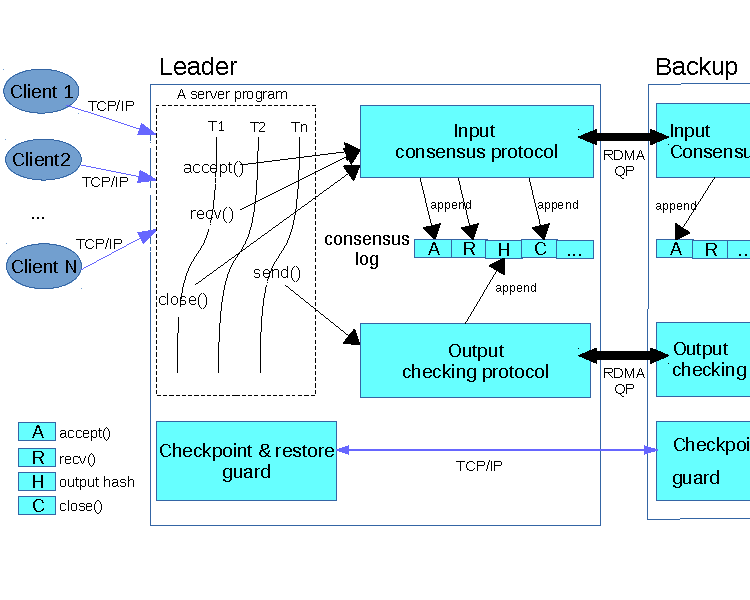
\includegraphics[width=0.5\textwidth]{figures/arch}
% \vspace{-.10in}
% \caption{{\em The \xxx Architecture.} \rm {\xxx components are shaded (and in
%   green).}} \label{fig:arch}
% \vspace{-.05in}
% \end{figure*}

% TBD. Input coordinator and output checker. Components.

% System model. Replicas. RDMA. LAN. Clients.
\xxx follows a typical \paxos runtime system 
deployment~\cite{scatter:sosp11,eve:osdi12,rex:eurosys14,crane:sosp15, 
dare:hpdc15}. It runs replicas of a server program in a datacenter. Replicas 
connect with each other using RDMA QPs. Client programs located in LAN or WAN. 
The leader handles client requests and runs our RDMA-based \paxos protocol to 
coordinate inputs among replicas.
% If a backup receives client 
% requests, it deny the requests and reply the leader's IP.

% \xxx intercepts four types of 
% socket operations: the \accept type, the \recv type, the \send type, and the 
% \close type. 
Figure~\ref{fig:arch} shows \xxx's architecture. \xxx intercepts a server 
program's socket calls (\eg, \recv) using a Linux technique called LD\_PRELOAD. 
\xxx involves four key components: a \paxos consensus protocol for input 
coordination (in short, the \emph{coordinator}), an output checking protocol 
(the \emph{checker}), a circular in-memory consensus log (the 
\emph{log}), and a guard process that handles checkpointing and recovering a 
server's process state and file system state (the \emph{guard}).

\begin{figure}[t]
\centering
\vspace{-.15in}
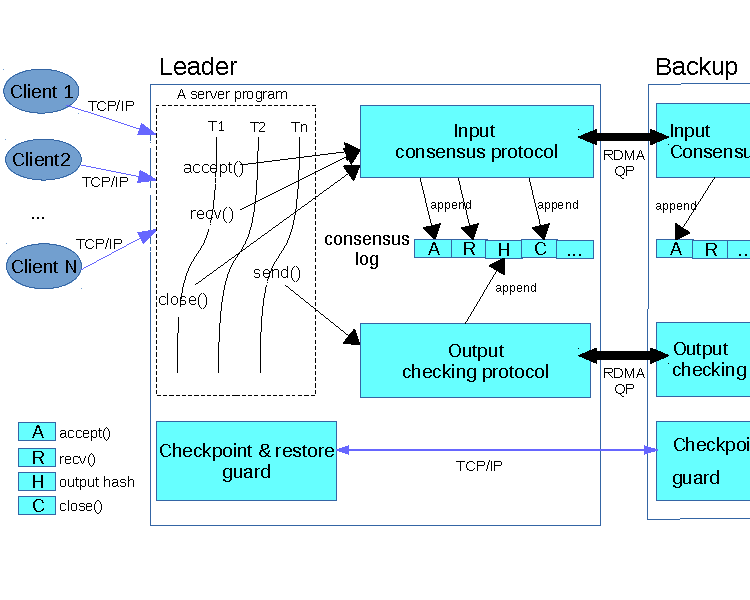
\includegraphics[width=.48\textwidth]{figures/arch}
\vspace{-.50in}
\caption{{\em The \xxx Architecture.} \xxx components are shaded (and in
  blue).}
\vspace{-.15in}
  \label{fig:arch}
\end{figure}


% Coordinator: leader side. 
The coordinator is invoked when a server program thread calls an inbound socket 
call to manage a client socket connection (\eg, \accept and \close) or to 
receive inputs from the connection (\eg, \recv). On the leader side, \xxx 
executes the actual Libc socket call, extracts the returned value or inputs of 
this call, stores it in local SSD, appends a log entry to its local consensus 
log, and then invokes the coordinator for a new consensus request on 
``executing this socket call".

The coordinator runs a consensus algorithm (\S\ref{sec:input}), which WRITEs 
the local entry to backups' remote logs in parallel and polls the local log 
entry to wait quorum. When a quorum is reached, the leader thread simply 
finishes intercepting this call and continues with its server execution. As 
the leader's server threads execute more calls, \xxx enforces the same 
consensus log and thus the same socket call sequence across replicas.

% In this request, in order tell the 
% backups what socket 
% calls they should execute, this request also carries the latest request 
% viewstamp that has reached consensus (\ie, the latest committed request).

% This coordinator invokes a consensus request by: (1) assigns this call a 
% monotonically increasing index (\ie, a viewstamp) in the log, (2) builds a 
% socket call struct (\S\ref{sec:input}), (3) store the struct to persistent 
% storage, (4) appends it to the log according to the index, and (5) writes this 
% struct to all remote backup replicas' log.

% Coordinator: backup side.
On each backup side, the coordinator uses a \xxx internal thread called 
\emph{follower} to poll its consensus log for new consensus requests. If the 
coordinator agrees the request, the follower stores the log entry in local SSD 
and then WRITEs a consensus reply to the remote leader's corresponding log 
entry. A backup does not need to intercept a server's socket calls because the 
follower will just follow the leader's consensus requests on executing what 
socket calls and then forward these calls to its local server program.

% To respond consensus requests rapidly, each 
% backup coordinator spawns a dedicated thread. This thread runs a busy loop to 
% pull consensus requests from the consensus log. This high-perfomance thread 
% runs in a spare dedicated CPU core and elinimates context switches, unlike 
% traditional TCP/IP that block threads socket calls to wait for requests.

% The backup 
% coordinator then forwards all the requests up to the latest committed socket 
% call to its local server process. 

% Consensus log. Same in both leader and backups.
% A consensus log appending operation is invoked whenever a leader's server 
% executes a socket call (except \send calls, handled by output checker). The 
% leader coordinator just appends socket calls to the log and backups follow 
% socket calls in this log.

% Output checker: leader side. % Output checker: backup side.
The output checker is occasionally invoked as the leader's server program 
executes outbound socket calls (\eg, \send). For every 1.5KB (MTU size) of 
accumulated outputs per connection, the checker unions the previous hash with 
current outputs and computes a new CRC64 hash. After a fixed number of hashes 
are generated, the checker then invokes consensus across replicas, which 
compares the hash at its global hash index on the leader side.

This output consensus is based on the input consensus algorithm 
(\S\ref{sec:input}) except that backups carry their hash at the same hash index 
back to the leader. For this particular output consensus, the leader first 
waits quorum. It then waits for a few \us in order to collect more remote 
hashes. It then compares remote hashes it has.

If a hash divergence is detected, the leader optionally invokes the local guard 
to forward a ``rollback" command to the diverged replica's guard. The diverged 
replica's guard then rolls back and restores the server program to a latest 
checkpoint before the last successful output check (\S\ref{sec:output}). The 
replica then restores and re-executes socket calls to catch up. Because output 
hash generations are fast and an output consensus is invoked occasionally, our 
evaluation didn't observe performance impact on this checker.

% Then, for every \emph{Tcheck} hash generations, the checker invokes a consensus 
% request on this hash value. This output consensus is the same as the 
% coordinator's input consensus except that backups' output checkers send ACKs 
% with their own hash values with the same index, whenever the hash values are 
% ready (some backups may run slowly). When a majority of hashes are back, the 
% leader's output checker compares these values and then makes an effort to roll 
% back divergent replicas to a previous checkpoint before the last matching hash. 


% Guard: leader side. % Guard: backup sides.
% Question: how does the backup replicas know the last matching hash? Through 
% committed viewstamp for the \send.
% The leader's guard accepts roll-back requests from the output checker and 
% forwards the requests to the corresponding guard on another, divergent repilca. 
% The divergent replca's guard then rolls back the server program to a previous 
% checkpoint before the last matching one, and then invokes the local input 
% coordinator to re-forward the requests in stable storage to the server. There 
% is no a second output hash comparisons between backups and leader until the 
% leader invokes a new output checking consensus request next time.


% \subsection{Example}\label{sec:example}
% 
% \begin{figure}[t]
% \centering
% \begin{minipage}{.5\textwidth}
% \lgrindfile{code/example.cpp.lineno}
% \end{minipage}
% \vspace{-.1in}
% \caption{{\em A server example.}} \label{fig:example}
% \vspace{-.20in}
% \end{figure}
% 
% \begin{figure}[t]
% \centering
% \begin{minipage}{.5\textwidth}
% \lgrindfile{code/client.cpp.lineno}
% \end{minipage}
% \vspace{-.1in}
% \caption{{\em A client example.}} \label{fig:client}
% \vspace{-.05in}
% \end{figure}

% TBD. A simple server with recv(), accept(), and send(). Must have a 
% concurrency bug in this toy program? Race on global var or heap?

% Describe the example code.
% Describe the example code. Describe a 'set' command from key-value store.
% Figure~\ref{fig:example} shows a simplified server code based on the \redis 
% key-value store, and Figure~\ref{fig:client} shows a client cocde. The server 
% accepts a new connection from a client, receives one input request, process the 
% request, and then sends a reply. Suppose the client sends a ``SET a b" request.

% Input coordination protocol.
% Once the client calls its \connect, the leader's server program calls the 
% \accept call intercepted by \xxx. The leader's input coordinator then invokes 
% consensus on building a new connection by writing a struct for \accept to 
% remote backups with RDMA. Once a majority of backups agree, the leader machine 
% returns from the \accept call and continues to run.

% When a client program calls its \send, leader's server traps into \xxx's \recv 
% function call, which a invokes consensus on this new input ``SET a b". If 
% a consensus is made by a majority of replicas, the leader directly returns from 
% \recv and processes the request, and each replica's dedicated thread sets up 
% a new connection to the local server because the \recv consensus request 
% notifies the backups that the last call, \accept, has reached consensus.


% Output checking protcol.
% Challenge: what if leader does more sends and replicas do fewer sends?
% When a request is processed and the server is about to send reply to the 
% client, \xxx traps into the \send call, computes historical hash value on 
% inputs when 4K bytes (MTU size). Since this request is short, no output check 
% will be invoked at this time. All backups return consensus reply to the leader 
% with their own hash values if this value is available on their replica. 
% Similarly, backups do the earlier socket call: the backups' follower forwards 
% ``SET a b" request to the local server program.

% TBD: explain why we do not need to intercept poll() function.

% TBD Question: must ask Cheng. The close logic is not clear. What do the 
% leaders and backups do for close()? Why do we have to need a NOP (if 
% backup thread does not close its connection to local server, it does not 
% matter, right)? 
% Finally, the leader's server program executes a \close call. Similarly, the 
% leader invokes consensus on this call, and the backups have this \close call in 
% their log so that they can close the 

% TBD: what is the interesting outcome of this program running with Falcon? 
% Replicating all inputs without modifications? Any chart figure/schedule? 
% Two points so far: automatically replicating all inputs without modification; 
% can tolerate one replica failure; the other two can still process requests.
\section{Input Consensus Protocol} \label{sec:input}

This section first presents \xxx's RDMA-accelerated \paxos consensus protocol, 
including the fast,scalable algorithm in normal case (\S\ref{sec:normal}), 
handling concurrent connections (\S\ref{sec:concurrent}), and the leader 
election protocol (\S\ref{sec:election}). It then analyzes the reliability of 
our protocol (\S\ref{sec:guarantees}).

\subsection{Normal Case Algorithm} \label{sec:normal}

\begin{figure}[t]
\centering
\begin{minipage}{.5\textwidth}
\lgrindfile{code/logentry.cpp}
\end{minipage}
\vspace{-.1in}
\caption{{\em \xxx's log entry for each socket call.}} \label{fig:logentry}
\vspace{-.05in}
\end{figure}

% \subsubsection{The Basic } \label{sec:primitive}

% Question: What if on a machine, it viewed it as the leader, it executes the 
% actual socket call, and then it invokes the consensus, but then it is no 
% longer the leader any more. How to undo the actual socket calls? Cases:
  %% On accept(). The old leader has already accepted and asks for consensus.
  %% On recv(). The old leader has already received.
  %% On send().
  %% On close().

% First, basic roles. log format details.
Recall that \xxx' input consensus protocol contains three roles. First, the 
\paxos consensus log (\S\ref{sec:overview}). Second, a leader replica's server 
program thread (in short, a leader thread) which invokes consensus request. For 
efficiency, \xxx lets a server program's threads directly handle consensus 
requests whenever they call inbound socket calls (\eg, \recv). Third, a backup 
replica's \xxx internal follower thread (\S\ref{sec:overview}) which agrees on 
or rejects consensus requests.

Figure~\ref{fig:logentry} shows the format of a log entry in \xxx's consensus 
log. Most fields are regular as those in a typical \paxos 
protocol~\cite{paxos:practical} except three ones: the \v{ack} array, the 
client connection ID \v{conn\_vs}, and the type ID of a socket call 
\v{call\_type}. The \v{ack} array is for backups to WRITE their consensus 
replies to the leader. The \v{conn\_vs} is for identifying which connection this 
socket call belongs to (see \ref{sec:concurrent}). The \v{call\_type} 
identifies four types of socket calls in \xxx: the \accept type (\eg, \accept), 
the \recv type (\eg, \recv and \myread), the \send type (\eg, \send and 
\mywrite), and the \close type (\eg, \close).

% Second, leader thread behavior on \recv(). Return from orig recv, grab 
% spin % lock and get view stamp, store the log, and post send to all replicas. 
% Non blocking. Wait % for over half agree, and then execute the operation.
Figure~\ref{fig:consensus} shows the input consensus algorithm. Suppose a 
leader thread invokes a consensus request when it calls a socket call with the 
\recv type. A consensus request includes four steps. The first step 
(\textbf{L1}) is executing the actual Libc socket call, because \xxx needs to 
get the actual return values or received data bytes of this call and then 
replicates them in remote replicas' logs.

\begin{figure}[b]
\centering
\vspace{-0.15in}
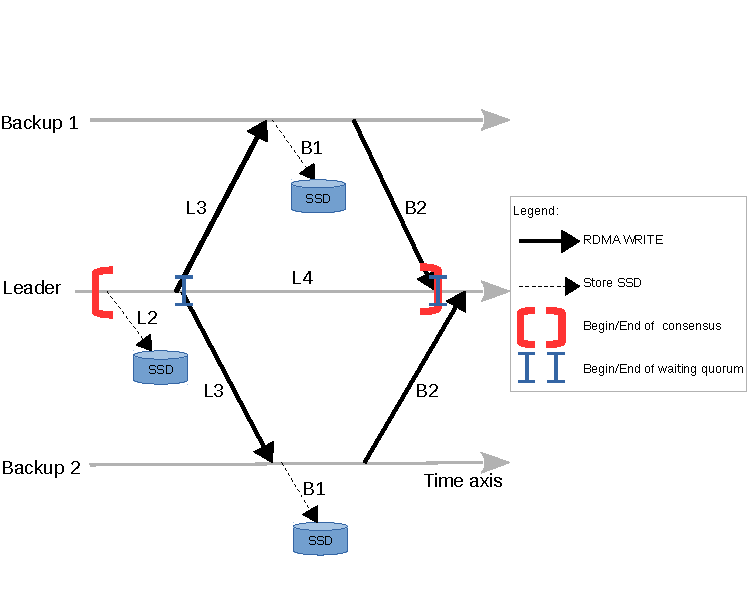
\includegraphics[width=.48\textwidth]{figures/consensus}
\vspace{-.4in}
\caption{{\em \xxx consensus algorithm in normal case.}} \label{fig:consensus}
\vspace{-.05in}
\end{figure}


The second step (\textbf{L2}) is local preparation, including assigning a 
global, monotonically increasing viewstamp to locate this entry in the 
consensus log, building a log entry structure for this call, and writing this 
entry to its local SSD.

The third step (\textbf{L3}) is to WRITE a log entry to remote backups 
in parallel. Unlike a previous RDMA-based consensus 
algorithm~\cite{dare:hpdc15} which has to wait for ACKs from remote NICs, our 
WRITE immediately returns after pushing the entry to its local QP between the 
leader and each backup, because \paxos has handled the reliability issues (\eg, 
packet losses) for our WRITEs. In our evaluation, pushing a log entry to local 
QP took no more than 0.1 \us. Therefore, the WRITEs to all backups are done in 
parallel (see \textbf{L3} in Figure~\ref{fig:logentry}).

% Instead, \xxx's leader thread just return 
% immediately after 
% putting the structs to the RDMA QP (Queue Pair) between a backup replica, 
% because \paxos protocol \xxx implements has already considered packet losses 
% (\eg, due to remote replica failures).

The fourth step (\textbf{L4}) is the leader thread polling on its \v{ack} 
field (notably, different from an RDMA ACK) in its local log entry for backups' 
consensus replies. Once consensus is reached, the leader thread finishes 
intercepting this \recv socket call and continues with its server application 
logic.

% 
% The leader does a
% busy loop to check the \v{ack} array until it sees that a majority of replicas, 
% including itself, have aggreed on this log entry. In normal case, both the 
% third and fourth steps will return immediately because no synchronization 
% context switch is involved.

% Post send carry the last committed (consensus reached) operation.

% One key issue, check integrity. Strawmen approach, check viewstamp first.
On a backup side, one tricky synchronization issue is that an efficient way is 
needed to make the leader's RDMA WRITEs and backups' polls atomic. For instance, 
while a leader thread is doing a WRITE on \v{vs} to a remote backup, this 
backup's follower thread may be reading this variable concurrently, causing a 
incomplete (wrong) read.

To address this issue, one existing approach~\cite{farm:nsdi14,herd:sigcomm14} 
leverages the left-to-right ordering of RDMA WRITEs and puts a special 
non-zero variable at the end of a fix-sized log entry because they mainly 
handle key-value stores with fixed value length. As long as this variable is 
non-zero, the RDMA WRITE ordering guarantees that the log entry WRITE is 
complete. However, because \xxx aims to support general server programs with 
largely variant received data lengths, this approach cannot be applied in \xxx.

Another approach is using atomic primitives provided by RDMA hardware, 
but a prior evaluation~\cite{drtm:sosp15} has shown that RDMA atomic 
primitives are much slower than normal RDMA WRITEs and local memory reads.
% Thus, in a RDMA-accelerated protocol, an extra mechanism 
% is needed to gurantee that a 
% leader's write has finished and then replicas can agree or disagree.

\xxx tackles this issue by adding a canary value after the actual \v{data} 
array. Because \xxx uses a QP with the type of RC (reliable connection) 
(\S\ref{sec:background}), the follower always first checks the canary value 
according to \v{data\_size} and then starts a standard \paxos consensus reply 
decision~\cite{paxos:practical}. Our efficient, synchronization-free approach 
guarantees that the follower always reads a complete log entry.
% This check guarantees that a log entry is 
% completely written in a local backup.
% 
% To ahchieve small consensus latency, \xxx's follower thread does a busy loop 
% on a dedicated CPU core to agree on consensus requests from the leader. Each 
% backup only needs one follower thread. This thread always busy reading the 
% latest un-agreed log entry in its local log, and it it sees a log entry has 
% completely written, it runs three steps. 

A follower thread in a backup replica polls from the latest un-agreed log 
entry and does three steps to agree on consensus requests, shown in 
Figure~\ref{fig:consensus}. First (\textbf{B1}), it does a regular \paxos view 
ID checking to see whether the leader is up-to-date, it then stores the log 
entry in its local SSD. Second (\textbf{B2}), it does a WRITE to send back 
a consensus reply to the leader's \v{ack} array element according to its 
own node ID. Backups perform these two steps in parallel 
(see Figure~\ref{fig:logentry}).

Third (\textbf{B3}, not shown in Figure~\ref{fig:consensus}), the follower 
does a regular \paxos check on \v{last\_committed} and executes all socket 
calls that it has not executed before this viewstamp. It then ``executes" each 
log entry by forwarding the socket calls to the local server program. This 
forwarding faithfully builds and closes concurrent connections between the 
follower and the local server program according to the socket calls in the 
consensus log.
% thus \xxx can 
% maintain consistent concurrent client connection mappings between the leader and 
% backups.


% TBD: should we put the impl here or somewhere else?
In a implementation level, \xxx stores log entries in local SSD using Berkley 
DB~\cite{berkeleydb}. Although \xxx's algorithm does not wait every RDMA ACK in 
order to achieve high scalability, we use selective signaling 
(\S\ref{sec:background}) to occasionally check and clear ACKs in the CQ 
associated with the QP, an essential ACK clearing step in RDMA implementations.

% On replicas, server programs run as is without being 
% intercepted. In short, this follower thread runs a high performance loop to 
% respond consensus requests and forward data to the local server program. Since 
% each backup machine only has one follower thread and nowadays machines often 
% have spare cores, we didn't find that the spin loop of this thread brought 
% bring negative performance impact in our evaluation.

% Performance: two RDMA writes and two SSD stores. No context switches.
% This protocol is highly optimized for minimizing consensus latency in normal 
% case. In total, a consensus between the leader and one backup only requires 
% two one-sided RDMA write operations (one from the leader to the backup and the 
% other from the backup to the leader) and two SSD write operations (each in 
% leader and backup). Although each RDMA one-sided operation takes about 3 \us, 
% \xxx's protocol just puts the log entry to the RDMA Queue Pair without needing 
% to wait until the write succeeds on the remote backup, because the leader will 
% have \paxos's consensus reply (the RDMA write from the backup to leader). In 
% addition, neither a leader thread or a follower thread does a synchronization 
% context switch during this consensus (a synchronization context switch 
% typically takes sub milli seconds, pretty slow).

% Question: one key question, can RDMA lose packets in between? I mean, both 
% data_size and canary value are correct, but packets in the middle are lost. 
% This may violate \paxos's non-corrupting packets assumption.

% Third, replica thread behavior on \recv(). Block on latest un agreed log, 
% wait for the % consensus log, check integrity, check view id, and then store to 
% BDB. and % then execute the committed but not executed requests from BDB.

\subsection{Handling Concurrent Connections} \label{sec:concurrent}

Unlike traditional \paxos protocols which mainly handle single-threaded 
programs due to the deterministic state machine assumption in SMR, \xxx aims to 
support both single-threaded as well as multithreaded server programs running 
on multi-core machines. Therefore, a strongly consistent mechanism is needed to 
map every concurrent client connection on the leader and to its corresponding 
connection on backups. A naive approach could be matching a leader connection's 
socket descriptor to the same one on a backup, but backups' servers may return 
nondeterministic descriptors due contentions on systems resources.

Fortunately, \paxos have already made viewstamps~\cite{paxos:practical} of 
socket calls strongly consistent across replicas. For TCP connections, \xxx 
adds the \v{conn\_vs} field, the viewstamp of the the first socket call in 
each connection (\ie, \accept) as the connection ID for log entries. Then, \xxx 
maintains a hash map on each local replica to map this connection ID to local 
socket descriptors.

% On a local 
% replica, \xxx maintains a hash map between this connection ID 
% to the actual local socket descriptor for each connection, then \xxx ensures 
% that data bytes are forwarded from a leader's connection to the right matching 
% connection on backups. \xxx also intercepts socket calls with the \close type 
% to clean up this map. For servers that use UDP to serve requests, \xxx maps the 
% viewstamp of a \recvfrom call to the socket descriptor returned from this call, 
% and it cleans up the map on a corresponding \sendto call. 

% TBD. Strawmen approach, use fds on leader machines.

%% thread ID mapping is not good too, because accept and recv can be called by 
% different threads in leader side.

% Use viewstamp of the accept() operation, consistent across replicas.


% What does replica thread do. High performance loop on a dedicated core.

\subsection{Leader Election} \label{sec:election}

% % Use one log operation or a few operations to do so. Clean, 
% match the PMS intention. Explain why this design choice is good.

% TBD. Four steps. Four entries?
Compared to traditional \paxos leader election protocols, RDMA-based 
leader election poses one main issue caused by RDMA. Because backups do not 
communicate frequently with each other in normal case, thus a backup does not 
know the remote memory locations where the other backups are polling. Writing to 
a wrong remote memory location may cause the other backups to miss all leader 
election messages. An existing system~\cite{dare:hpdc15} establishes an extra 
control QP with extra remote memory to handle leader election, posing more
complexity via the extra communication channels.

% If current leader fails, 
% how does a backup know the other remote backups' memory location to WRITE to? 

% Mention old leader.
% The second issue still stems from RDMA's nature: while a leader election is 
% on going, the out-dated leader may still WRITE to remote backups and corrupt 
% the ongoing leader election. This WRITE will not get a Yes consensus reply 
% because the other replicas can transit their current state from active to a 
% leader election state~\cite{paxos:practical}, but the old leader's WRITE may 
% still corrupt the ongoing leader election. 

\xxx addresses this issue with a simple, clean approach. It runs election 
election with the same consensus log and the same QP. In normal case, the leader 
does WRITEs to remote logs as heartbeats with a period of T. Each consensus log 
maintains a control data structure called \v{elect[MAX]}, one element for each 
replica. Normal case operations and heartbeats use the other parts of the 
consensus log but leave this \v{elect} array alone. Once backups have not 
received heartbeats from the leader for a period of 3*T, they start to elect a 
new leader and let their follower threads poll from the \v{elect} array.

% Before starting a standard leader election 
% phase as in traditional \paxos protocols~\cite{paxos:practical}, each backup 
% always first does RDMA one-sided reads to get remote replicas' current polling 
% location.

Backups start a standard \paxos leader election 
algorithm~\cite{paxos:practical} with three steps. Each replica writes to its 
own \v{elect} element at remote replicas. First, backups propose a new view 
with a standard two-round \paxos consensus~\cite{paxos:simple} by including its 
current log entry offset. The other backups also propose their views and poll 
on this array in order to follow other proposals or confirm itself as the 
winner. The backup with largest log offset will win. Second, the winner 
proposes itself as a leader candidate using this array, another two-round 
\paxos consensus. Third, after the second step reaches a quorum, the new leader 
notifies remote replicas itself as the new leader and it starts to WRITE 
periodic heartbeats.

\subsection{Reliability} \label{sec:guarantees}

% Follow PMP, ease to understand, absorbe good exeprience.
% \paxos is notoriously difficult to 
% understand~\cite{raft:usenix14,paxos:simple,paxos,paxos:complex} or 
% implement~\cite{paxos:live,paxos:practical}. 
% 
To minimize protocol-level bugs, 
\xxx's \paxos protocol mostly sticks with a popular, 
practical implementation~\cite{paxos:practical}, especially the behaviors of 
senders and receivers (\S\ref{sec:normal} and \S\ref{sec:election}). For 
instance, both \xxx's normal case algorithm and 
the popular implementation~\cite{paxos:practical} involve two messages and 
same senders and receivers (although we use WRITEs and carefully make them run 
in parallel). We made this choice 
because \paxos is \paxos is notoriously difficult to 
understand~\cite{raft:usenix14,paxos:simple,paxos,paxos:complex} or 
implement~\cite{paxos:live,paxos:practical} 
verify~\cite{modist:nsdi09,demeter:sosp11}. Aligning with a practical
\paxos implementation~\cite{paxos:practical} helps us incorporate these 
readily mature understanding, engineering experience, and the theoretically 
verified safety rules into our protocol design and implementation.

% TBD: reliability analyzes. We do not need the lossless assumption in RDMA QPs.
Although \xxx's \paxos protocol works on a RDMA network, the reliability of 
this protocol does not rely on the lossless networking in RDMA. \xxx's protocol 
still complies with the standard \paxos failure-handling model, where a stable 
storage exists, but hardware may fail, network may be partitioned, packets may 
be delayed or lost, and server programs may crash.


% Define safety: TBD.
% A \paxos protocol must ensure safety: the agreed operation must be an actually 
% proposed one; if agreed, all active replicas must consistently enforce this 
% operation. Safety is another important sweet spot that \xxx's input 
% coordination protocol inherites from traditional \paxos protocol by sticking 
% with same replica behavior in traditional ones. As a traditional protocol, 
% our input coordination protocol also uses view IDs and viewstamps to enforce a 
% consistent, up-to-date leadership across replicas. To address the atomicy issue 
% between remote RDMA writes and local memory reads, our protocol addes an 
% completion check on log entries (\S\ref{sec:normal}).
% In short, our 
% design choice makes our input coordination protocol enforce the same level of 
% safety as traditional \paxos protocols~\cite{paxos, paxos:simple, 
% paxos:practical}.

% Safety, viewstamp.

% Store to stable storage.

% Any unique changes that prevent us from providing guarantees? The delta 
% changes? Packets. Logs?

% \begin{figure}[t]
% \centering
% \vspace{-.20in}
% 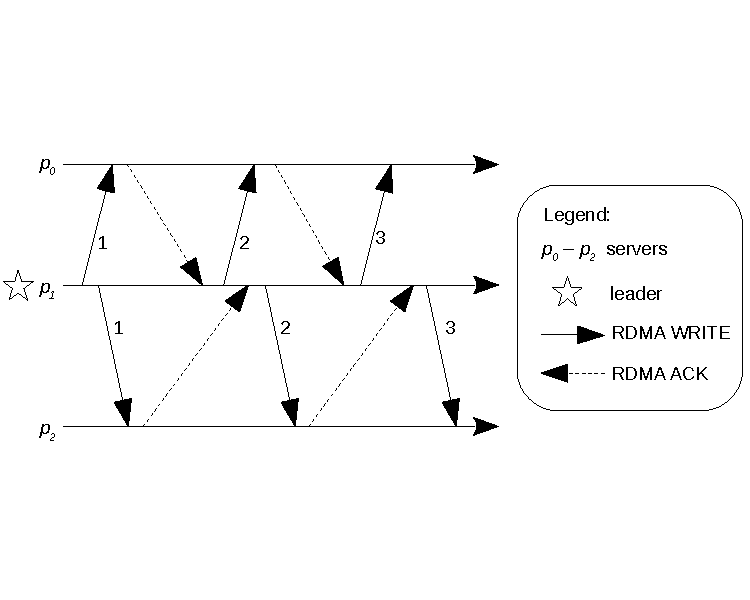
\includegraphics[width=.48\textwidth]{figures/dare}
% \vspace{-.20in}
% \caption{{\em DARE consensus algorithm in normal case.}} \label{fig:dare}
% \vspace{-.05in}
% \end{figure}
% 
% We compare the performance and scalability between \xxx and DARE, the fastest 
% RDMA-based consensus algorithm we know so far. As shown on 
% Figure~\ref{fig:consensus}, a complete \xxx consensus round consists of three 
% parts: a leader's local SSD store operation (L2), a backup's local SSD store 
% operation (B1), and a WRITE round-trip (L3 and B2). Given the same inputs, 
% the latency of these three parts are constant, thus \xxx's consensus latency is 
% not approximately constant to replica group size. \xxx's scalability is mainly 
% bounded by the max number of outbound RDMA writes in the RDMA NIC hardware 
% (currently, 16~\cite{herd:sigcomm}).
% 
% We carefully examined DARE's code base and depict its consensus algorithm in 
% Figure~\ref{fig:dare}, which consists of three parts: log entry WRITEs to all 
% remote logs' with ACKs, log tail pointer WRITEs to all remote logs with ACKs, 
% and a quorum notification by WRITEs to agreed remote replicas without ACKs. In 
% DARE's pure leader-based consensus, ACKs are necessary for every next step to 
% start. Therefore, DARE's consensus latency is linear to replica group size. We 
% show concrete consensus latency comparisons of \xxx and DARE in evaluation 
% (\S\ref{sec:scalability}).
\section{Output Checking Protocol} \label{sec:output}

% TBD. Motivation of this approach. Make replicas follow consistent execution 
% states. Recover from bugs that diverge executions. 
This section presents \xxx's output checking protocol for detecting and 
recovering from replicas' execution divergence. This section first introduces 
how \xxx computes and compares network outputs among replicas 
(\S\ref{sec:output-workflow}), and then introduces its checkpoint and rollback 
mechanism to deal with divergence (\S\ref{sec:checkpoint}).

\subsection{Computing and Comparing Network Outputs} \label{sec:output-workflow}

% Main issue. Output timings are pretty miscellaneous.
One main issue on checking network outputs is the physical timing when a 
server program produces an network output is usually miscellaneous. For 
example, when we ran \redis simply on pure SET workloads, we found that 
different replicas reply the numbers of ``OK" replies for SET operations 
randomly: one replica may send four of them in one \send call, while another 
replica may only send one of them in each \send call. Therefore, comparing 
outputs on each \send call among replicas may not only yield wrong results, but 
may unnecesssarily slow down server programs among replicas.

% Two variables. Tckpt (checkpoint periods) and Tcmp (comparison periods).
To overcome this timing issue, \xxx presents a bucket-based hash computation 
mechanism. When a server calls a \send call, \xxx puts the sent bytes into a 
local, per-connection bucket with 1.5KB (same as MTU size). Whenever a bucket 
is full, \xxx computes a new CRC64 hash on a union of the current hash and this 
bucket. Such a hash computation mechanism encodes accumulated network outputs. 
Then, after every \thashcomp (by default, 1000 in \xxx) local hash values are 
generated, \xxx invokes a output checking protocol to check this hash across 
replicas. The index of this hash in the generated sequence is consistent across 
replicas because each replica runs the same mechanism to generate the hash 
sequence.

% TBD. Briefly describe why using our input coordination protocol for output 
% checking is good. Simply the whole system, reliable (tolerate packet 
% lossses and consistency, thanks to paxos), fast, already have ACK mechanisms.

% Leverage the input protocol to carry the hash of outputs. Occasionally.
To compare a hash across replicas, \xxx's output checking protocol runs the 
same as the input coordination protocol (\S\ref{sec:normal}) except that the 
follower thread on each backup replica carries this hash value in the \v{ack} 
written back into the leader's corresponding log entry. To make an effort to 
collect more remote hash values, \xxx waits for \twait (by default, 20 \us) 
and then starts to detect divergence on hash values.

% This output protocol starts by letting a leader thread invoke a consensue 
% request on this hash comparison for its own client connection. The leader also 
% writes its own hash value in the \v{ack} array with its own replica ID. Then, 
% follower threads on backup replicas carry their local hash values in the \v{ack} 
% array according to the connection ID \v{conn\_vs}. Once a quorum of \v{ack} 
% is ready, the leader simply detects divergence with the hash values in its 
% local \v{ack} array. Note that at this moment, some replicas may not send back 
% their reply yet because only a quorum is reached. To make an effort to collect 
% a complete hash values, \xxx waits for \twait (by default, 20 \us) and then 
% starts to detect divergence on hash values.

Figure~\ref{fig:divergence} shows the workflow on how the leader checks 
present replies and handles divergence, which include four possible cases: 
(1) all hashes are the same; (2) leader's hash equals a majority of replicas, 
but minor replicas' hashes diverge; (3) leader's hash diverges from a majority 
of replicas'; and (4) no majority has the same hash value. The first three 
cases should be the normal case unless a program tends to frequently compute 
outputs on random functions (\eg, a scientific similator).

Note that \xxx does has incorporated an input re-planing approach (\eg, 
Eve~\cite{eve:osdi12} sequentially re-execute requests after a rollback) because 
we found that simply re-execution can already avoid the divergence. Previous 
work~\cite{lu:concurrency-bugs,pres:sosp09} also confirmed that it was 
extremely unlikely to trigger a concurrency bug in both of two consencutive 
executions.

% Even so, we can 
% leverage prior approaches to hook these 
% random functions~\cite{paxos:practical,eve:osdi12} and make them generate same 
% return values among replicas.

% Once the leader decides to roll back a diverged replica (including itself), it 
% invokes a local guard process (\S\ref{sec:overview}) that handles 
% checkpointing and rolling back the local server program. If a remote replica 
% needs to be rolled back, the local guard forwards the roll back request to the 
% guard in that remote replica.
% 
% We explicitly design this output checking protocol to be fast with two 
% considrations: (1) because the hash comparison consensus happens occasionally 
% (every \thashcomp hash generations), the performance penalty on this output 
% consensus is negligible; and (2) all or most replicas' hash values are 
% the same in normal case. Two parameters, \thashcomp and \twait, may be 
% sensitive to \xxx's performance. We did an evaluation on diverse server 
% programs and found that these default values are reasonable, general settings to 
% these programs (\S\ref{sec:sensitivity}).

% When divergence is detected, spawn the mechanism, show workflow.

% Strawmen approach? Necessary?

\begin{figure}[t]
\centering
\vspace{-.10in}
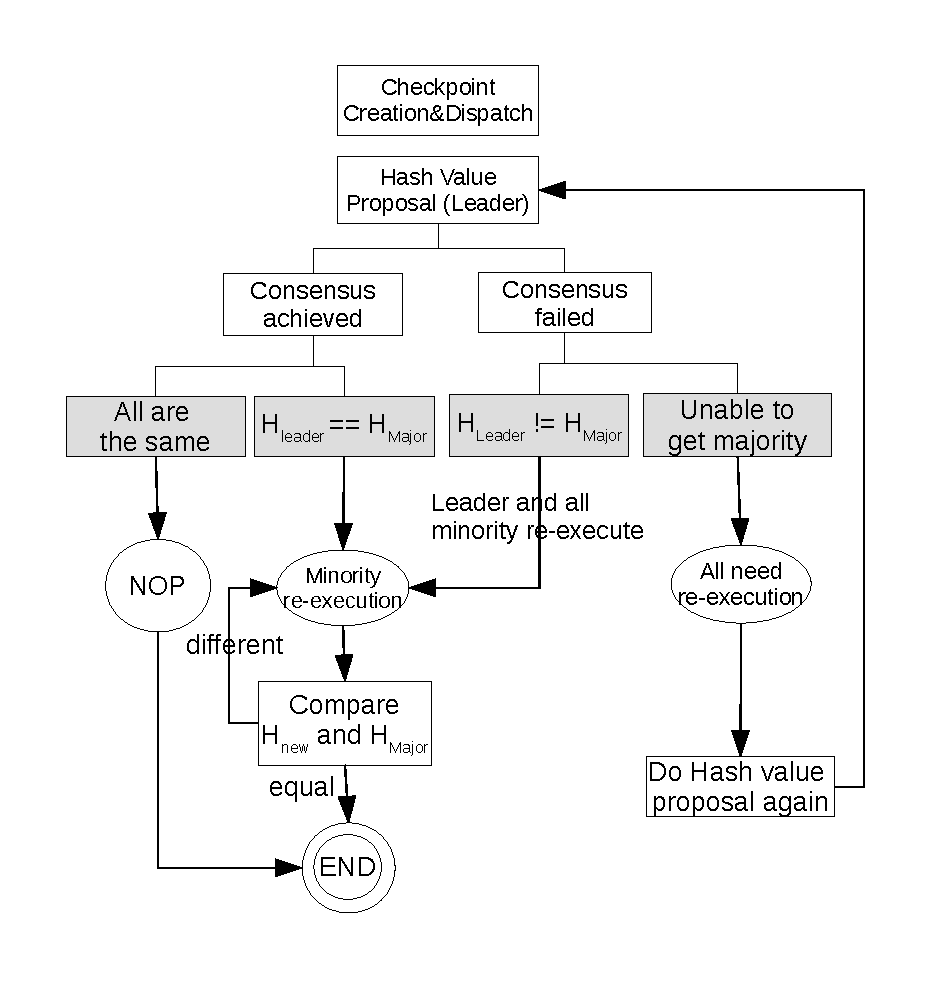
\includegraphics[width=.5\textwidth]{figures/output-divergence}
\vspace{-.50in}
\caption{{\em Workflow to Handle Network Output Divergence.}} 
\label{fig:divergence}
\vspace{-.20in}
\end{figure}

\subsection{Checkpoint and Restore Implementations} \label{sec:checkpoint}

% Regularly: periodically checkpoint. Contain both process state and file 
% system state, so that we do not need to check output to file system.
A guard process is running on each replica to checkpoint and restore the local 
server program. The guard does two tasks. First, \xxx assigns one backup 
replica's guard to checkpoint the local server program's process state and file 
system state of current working directory within a physical duration 
\tcheckpoint (by default, one hour in \xxx).

Such a checkpoint operation and its duration are not sensitive to \xxx's 
performance because the other backups can still reach quorum rapidly. Each 
checkpoint is associate with a last committed socket call viewstamp of the 
server program. After each periodical checkpoint, the backup distributes the 
checkpoint zip file to the other replicas.

Specifically, \xxx leverages CRIU, a popular, open source process checkpoint 
tool, to checkpoint a server program's process state (\eg, CPU registers and 
memory). Since CRIU does not support checkpointing RDMA connections, \xxx's 
guard first sends a ``close RDMA QP" request to an \xxx internal thread, lets 
this thread closes all remote RDMA QPs, and then invokes CRIU to do the 
checkpoint.

The second task for guards is that all guards in all alive replicas handle 
rollback requests once divergence is detected (\S\ref{sec:output-workflow}). 
According to the rollback workflow, a backup guard which receives a rollback 
request from the leader guard will kill the local server process and roll back 
to a previous checkpoint before the last successfuly hash check.
% Suppose the 
% viewstamp associated with the 
% % previous checkpoint is $vs_{ckpt}$, and the viewstamp of the last matching 
% hash 
% % comparison log entry is $vs_{match}$, \xxx ensures that $vs_{ckpt}$ 
% % is smaller than $vs_{match}$ so that this checkpoint is not diverged.

% After checkpointing process state, \xxx uses CRIU to stop this process and then 
% zip files in the process's current working directory recursively, including the 
% socket call stable storage (\S\ref{sec:input}). In our evaluation, 
% zipping current working directory was sufficient to carry all files used 
% by the evaluated programs.

% To avoid a server 
% to modify files missed by \xxx, we only assign a server process write 
% permissions to its current working directory and the ``/tmp" directory (files in 
% ``/tmp" directory often do not matter). \xxx's file system checkpoint avoids the 
% need of comparing program outputs to the file system.

% Closing RDMA sockets before checkpoint because CRIU does not support such 
% special memory.



% Orthogonal to the \paxos protocol, just feel like some replicas restart 
% themselves. Paxos can handle this.

% Sound. As long as local machines have a checkpoint with a viewstamp before 
% the last matched output check.

% Closing RDMA sockets before checkpoint because CRIU does not support such 
% special memory.


% \subsection{Efficiency and Reliability} \label{sec:output-discuss}
% % Efficient. Occasionally check hash. 
% 
% % Sound. If Tckpt is longer than Tcomp.



\section{Checkpoint and Restore} \label{sec:checkpoint}

TBD.
\section{Implementation Details} \label{sec:impl}

This section first presents our parallel input logging mechanism 
(\S\ref{sec:logging}) for storing inputs efficiently, and then our 
checkpoint/restore mechanism for recovering and adding replicas 
(\S\ref{sec:checkpoint}).

\subsection{Parallel Input Logging} \label{sec:logging}

To handle replica fail-overs, a standard \paxos protocol should provide a 
persistent input logging storage. \xxx uses the \paxos viewstamp of each input 
as key and its input data as value. \xxx stores this key-value pair in 
Berkeley DB (BDB) with a BTree access method~\cite{berkeleydb}, because found 
this method fastest in our evaluation.

However, if more inputs are inserted, the BTree height 
will increase, which will cause the key-value insertion latency to 
largely increase.

To handle this issue, we implemented a thread-safe, 
parallel logging approach~\cite{Bessani:usenix13}: instead of maintaining a 
single BDB store, we maintain an array of BDB stores. We use an index to 
indicate the current active store and insert new inputs. Once the number of 
insertions reach a threshold, we move the index to the next empty store in the 
array and recycle the preceding stores. This Implementation efficiently kept our 
input logging latency within 2.8$\sim$8.7 \us (\S\ref{sec:overhead}).

\subsection{Checkpoint and Restore} \label{sec:checkpoint}

We proactively design \xxx's checkpoint mechanism to incur little performance 
impact in normal case. A checkpoint operation is invoked periodically 
in one backup replica, so the leader and other backups can still reach 
consensus on new inputs rapidly.

% Regularly: periodically checkpoint. Contain both process state and file 
% system state, so that we do not need to check output to file system.
A guard process is running on each replica to checkpoint and restore the 
local server program. It assigns one backup 
replica's guard to checkpoint the local server program's process state and file 
system state of current working directory within a one-minute duration.

Such a checkpoint operation and its duration are not sensitive to normal case
performance because the other backups can still reach quorum rapidly. Each 
checkpoint is associate with a last committed socket call viewstamp of the 
server program. After each checkpoint, the backup dispatches the checkpoint zip 
file to the other replicas.

Specifically, \xxx leverages CRIU, a popular, open source process checkpoint 
tool, to checkpoint a server program's process state (\eg, CPU registers and 
memory). Since CRIU does not support checkpointing RDMA connections, \xxx's 
guard first sends a ``close RDMA QP" request to an \xxx internal thread, lets 
this thread closes all remote RDMA QPs, and then invokes CRIU to do the 
checkpoint.

% The second task for guards is that all guards in all alive replicas handle 
% rollback requests once divergence is detected (\S\ref{sec:output-workflow}). 
% According to the rollback workflow, a backup guard which receives a rollback 
% request from the leader guard will kill the local server process and roll back 
% to a previous checkpoint before the last successful hash check.




\section{Discussions}\label{sec:discuss}
% 
This section compares \xxx and \dare's protocols (\S\ref{sec:compare}), and 
discusses \xxx's limitations (\S\ref{sec:limits}) and its broad application 
areas (\S\ref{sec:apps}).

\subsection{Comparing \xxx and \dare}\label{sec:compare}

\begin{figure}[t]
\centering
\vspace{-.5in}
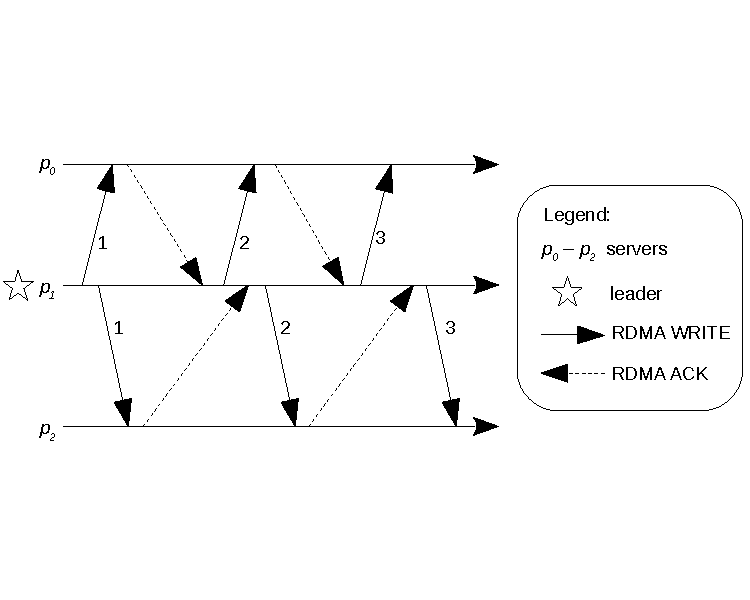
\includegraphics[width=.35\textwidth]{figures/dare}
\vspace{-.6in}
\caption{{\em \dare's RDMA-based protocol.} This is a sole-leader, 
two-round protocol with three steps: (1) the leader WRITEs a consensus request 
to all backups' consensus logs and waits for ACKs to check if they succeed; 
(2) for the successful backups in (1), leader does WRITEs to update tail 
pointer of their consensus logs; and (3) on receiving a majority of ACKs in (2), 
a consensus is reached, leader does WRITEs to notify backups without needing to 
wait ACKs.}
\label{fig:dare}
\vspace{-.20in}
\end{figure}

We highly appreciate \dare~\cite{dare:hpdc15}, the first RDMA-based, 
\paxos-like protocol. It is most relevant to \xxx. To tolerate single point of 
program failures, \dare is designed to run with a small (three to five) replica 
group. Under this design choice, \dare's protocol is sole-leader (backups do 
not participate in consensus): the leader only needs to do two-round WRITEs and 
check the ACKs of these WRITEs for a consensus. Figure~\ref{fig:dare} shows 
\dare's protocol.

% 
% logic uses two rounds to  wait for RDMA ACKs from backups. Our evaluation 
% shows that this protocol is fast when replica group size is small (three to 
% five), but both the ACK pollings and two-round

% It is a 
% sole-leader protocol (backups do not participate in consensus) with two rounds. 
% In the first round, the leader uses RDMA to write the consensus requests to all 
% replicas and polls RDMA ACKs to check whether the writes succeed. Second, for 
% the successful writes, the leader does another round of RDMA writes to mark the 
% writes as successful on other replicas, and poll ACKs on these writes. Once a 
% majority of successful writes in the second round, DARE reaches a consensus.

To further improve performance, \dare makes two technical choices. First, to 
avoid delays caused by polling ACKs, \dare uses a global RDMA CQ (Completion 
Queue) for all replicas, making it possible to collect multiple ACKs each poll 
operation. Second, this protocol does not incorporate a persistent storage or 
checkpoint/restore design. Therefore, \dare lacks durability 
(\S\ref{sec:background}), an important guarantee in traditional \paxos 
protocols and in \xxx.

% With these 
% two choices, \dare runs slightly faster than \xxx on three replicas.

However, \dare is not designed to scale to a large replica group. Our 
evaluation shows that both \dare's ACK pollings and its two-round consensus 
incurred scalability bottle approximately linearly consensus latency: DARE's 
consensus latency increased by \darescalability as replica group 
size increased by 35x (\S\ref{evaluation}).

Overall, \xxx differs from \dare in three aspects. First, \xxx is a one-round 
protocol, while \dare has two rounds. To achieve one-round consensus, \xxx's 
backups poll from its local memory to receive consensus requests, so \xxx 
consumes more CPU than \dare on backlups. Second, \xxx has shown to scale well
(sub-linearly) on 100+ nodes (\S\ref{sec:comp-dare}), while \dare did not 
discuss their scalability in paper. Third, to ensure durability, \xxx's 
protocol includes a persistent storage.

\subsection{\xxx Limitations}\label{sec:limits}

% Input coordination protocol.

% Have not hooked time and rand(). Can use PMP approach. Not a problem for 
% evaluated apps. 
\xxx currently does not hook random functions such as \v{gettimeofday()} and 
\v{rand()} because these random results are often explicit and easy to examine 
from network outputs (\eg, a timestamp in the header of a reply). Existing 
approaches~\cite{eve:osdi12,paxos:practical} in \paxos protocols can also be 
leveraged to intercept these functions and make them produce same results among 
replicas.
% because our output checkers have not detected network output 
% divergence comming from these functions

% Output checking protocol.

% Clamav style.
\xxx's output checking protocol may have false positives or false negatives, 
because it is just designed to try to improve assurance on whether replicas run 
in sync. A server program running in \xxx may have false positive when it uses 
multiple threads to serve the same client connection and uses these threads to 
concurrently add outputs (\eg, \clamav in our evaluation). 
Running a deterministic multithreading 
scheduler~\cite{coredet:asplos10,parrot:sosp13} with the server program 
addresses this problem.
% In our evaluation, all programs except \clamav uses only 
% one thread to process one client connection and they don't have such false 
% positives.

A server program may also have false negative when it triggers a software bug 
but the bug does not propagate to network outputs. From client programs' point 
of view, such bugs do not matter. Moreover, \xxx already checkpoints file 
system state to mitigate this issue.

Currently \xxx has not incorporated read-only optimization~\cite{eve:osdi12} 
because its performance overhead compared to the evaluated programs' 
unreplicated executions is already reasonable (\S\ref{sec:overhead}). However, 
\xxx can be extended to support read-only optimization if two conditions are 
met: (1) whether the semantic an operation is read-only is clear in a server 
program; and (2) the number of output bytes for this operation is fixed. GET 
requests in key-value stores often meet these two conditions.

We use GET requests to present a design. \xxx intercepts a client program's 
outbound socket calls (\eg, \send), compares the first three bytes in each call 
with ``GET". If they match, \xxx appends two extra \xxx metadata fields 
\v{read\_only} and \v{length} in this outbound call to the server. \xxx then 
intercepts a server's \recv calls and strips these two fields. If the first 
field is true, \xxx directly processes this operation in a local replica 
and strips the next \v{length} bytes from the output checker within the same
connection. In sum, \xxx processes these operations locally without making 
outputs across replicas diverge.

% When execution divergence is detected in a replica, \xxx's rollback mechanism 
% is not designed to guarantee that the re-executions of this replica will 
% definitely avoids this divergence. We made this design choice because both 
% our evaluation and a previous work Eve~\cite{eve:osdi12} found that divergence 
% happens extremely rarely in evaluation. In our evaluation, we found that simply 
% re-executing the log can practically make \xxx's replicas converge to 
% same execution states. A similar finding is that although Eve provided a 
% sequential re-execution approach to with divergence avoidance guarantee, which 
% \xxx can leverage, but even Eve's evaluation didn't experience any divergence 
% and thus this approach was not invoked.

% Read only opt?

% No guarantees on recovery. Best effort. But, can we actually server requests 
% one by one?

%% No lxc.

%% Support for Java may not be good due to the VM memory copying. Some 
% techniques that avoid memory copying may be usable~\cite{weixu:tsinghua}. Good 
% for % C/C++ programs as long as they use POSIX socket APIs.



\subsection{\xxx Has Broad Applications}\label{sec:apps}

In addition to greatly improving the availability of general server programs, 
we envision that \xxx can be applied in broad areas, and here we elaborate 
three. First, \xxx's RDMA-accelerated \paxos protocol and its implementation 
could be a template for other replication protocols (\eg, byzantine 
fault-tolerance~\cite{zyzzyva:sosp07,pbft:osdi99}). 

% Another promising direction is three-phase commit (3PC): 3PC is often 
% blamed by its intolerance on network partitions and asynchronour 
% communications, 
% and its high latency caused by the three round-trips. Fortunately, within the 
% RDMA-enabled datacenter context, people may leverage \xxx's techniques and 
% experience to build a significantly faster and more reliable 3PC protocols.

% Other replication topics.

% Parallel program analysis. Such a short coordination time can make replicas 
% run almost as fast as each other, support many time-critical analyses 
% such as race detection and security defenses.
Second, by efficiently constructing multiple, equivalent executions for the 
same program, \xxx can benefit distributed program analysis techniques. Bounded 
by the limited computing resources on single machine, recent advanced 
program analysis frameworks become 
distributed~\cite{decouple:usenix08, speck:asplos08, 
shadowreplica:ccs13, wester:parallelizing:asplos13,repframe:apsys15} in order to 
offload analyses on multiple machines. \xxx can be leveraged in these 
frameworks so that developers of analysis tools can just focus on their own 
analysis logic, while \xxx's general replication architecture handles the rest.

Moreover, program analyses developers can tightly integrate their tools with 
\xxx. For instance, they can proactively diversify the orders of socket calls 
in \xxx's consensus logs among replicas to improve replicas' tolerance on 
security attacks~\cite{con:hotpar12}.

% TBD: use \xxx to detect software bugs by checking outputs, even in 
% real-world deployments. XXX make program % inputs strongly consistent across 
% replicas, so output divergence are likely % from software bugs. XXX promising 
% 
% results in our evaluation. Find a bug in % ssdb?

% One idea: can leverage the checkpoint and rollback protocok, and the 
% consensus part, to build a system that can automatically bypass concurrency 
% bugs without fixing them. The way to bypass: proactively reordering socket 
% calls. Self-healing system.

% A core building block in future operating systems. Maintain a consistent view 
% of computing resources and data. Used in scheduling framework (Mesos) because 
% its latency is almost compatible with context switches of processes (sub 
% milli seconds).
Third, \xxx can be a core building block in the emerging datacenter operating 
systems~\cite{matei:hotcloud11, mesos:nsdi11, datacenter:os}. As a 
datacenter continuously emerges a computer, an OS may be increasingly needed for 
such a giant computer. \xxx's fast, general coordination service is especially 
suitable for such an OS's scheduler to maintain a consistent, reliable view on 
both computing resources and data in a datacenter. For instance, \xxx's 
latency is largely between less than 30 \us, much smaller than a typical 
process context switch (a few hundreds \us).

\section{Evaluation} \label{sec:evaluation}

Our evaluation used three Dell R430 servers as replicas. Each server having 
Linux 3.XX.X, 2.6 GHz Intel Xeon CPU with 24 hyperthreading cores, 32GB memory, 
and 1T SSD. Each machine has a Mellanox ConnectX-3 Pro Dual Port 40 Gbps NIC. 
These NIC are connected using the InfiniBand RDMA architecture through a Dell 
S6000 high-performance switch with 32 40Gpbs ports. The price of these 
RDMA-relevant hardware were moderate: each server costs US \$5,328 and the 
switch costs US \$12,894.

We evaluated \xxx on \nprog server programs, including \redis, 
\memcached, \ssdb, and \mongodb, \nkvprog key value stores; \mysql, a SQL 
server; \clamav, a anti-virus server that scans files and delete malicious 
ones; \mediatomb, a multimedia storage server that stores and transcodes video 
and audeo files; \openldap, a LDAP server, \tftp, a FTP server. In addition 
to these widely used \npopularprog programs, We have also evaluated \calvin, an 
advanced transactional database system that leverages \zookeeper as its SMR 
service. All these programs are multithreaded except \redis (but it can still 
serve requests concurrently using Libevent). These servers all process, 
update, and store important data and files, thus the high fault-tolerance of SMR 
is especially attractive to these programs.

\begin{table}[b]
\footnotesize
\centering
\vspace{-.05in}
\begin{tabular}{lrr}
{\bf Program} & {\bf Benchmark} & {\bf Benchmark workload description}\\
\hline\\[-2.3ex]
\clamav & Self  & Scan files in /usr/lib directory \\
\mediatomb & ApacheBench  & Transcode video files in parallel\\
\memcached & mcperf  & Half set and half put\\
\mongodb & YCSB  & Workload C\\
\mysql & Sysbench  & Concurrent SQL transactions\\
\openldap & Self  & \openldap's test program\\
\redis & Self  & Half set and half put\\
\ssdb & Self  & Half set and half put\\
\calvin & Self  & Concurrent SQL transactions\\
\end{tabular}
\vspace{-.05in}
\caption{{\em Benchmarks and workloads.} ``Self" in the Benchmark column means 
we used the server's own performance benchnmark.} 
\label{tab:benchmarks}
\end{table}


% Benchmarks table.
To evaluate the \xxx's practicality, we used popular third-party or the 
developers' own performance benchmarks for all these servers. For benchmark 
workload settings, we used the benchmarks' default workloads whenever 
available. Table~\ref{tab:benchmarks} introduces the benchmarks and workloads 
we used. To mitigate network latency of public network, all benchmarks were 
ran in a Dell R320 server, with Linux 3.XX.X, 2.2GHz Intel Xeon with 12 
hyperthreading cores, 16GB memory, and 160G SSD. This server connects with the 
replica machines with 1GBps 1Gbps bandwidth LAN, with a mean 401 \us ping 
round-trip latency. A larger latency (\eg, running clients from WAN) will 
further mask \xxx's overhead. We spawned up to 16 concurrent connections 
which made these servers reached peak throughput, and then we measured both 
response time (latency) and throughput. We also measured \xxx's bare 
latency on consensus. Each performance data point in the evaluation is taken 
from the mean value of 10 repeated executions.

% evaluation metric. client benchmarks all run in LAN, average latency



\subsection{Performance Overhead} \label{sec:overhead}

\begin{figure*}[t]
\centering
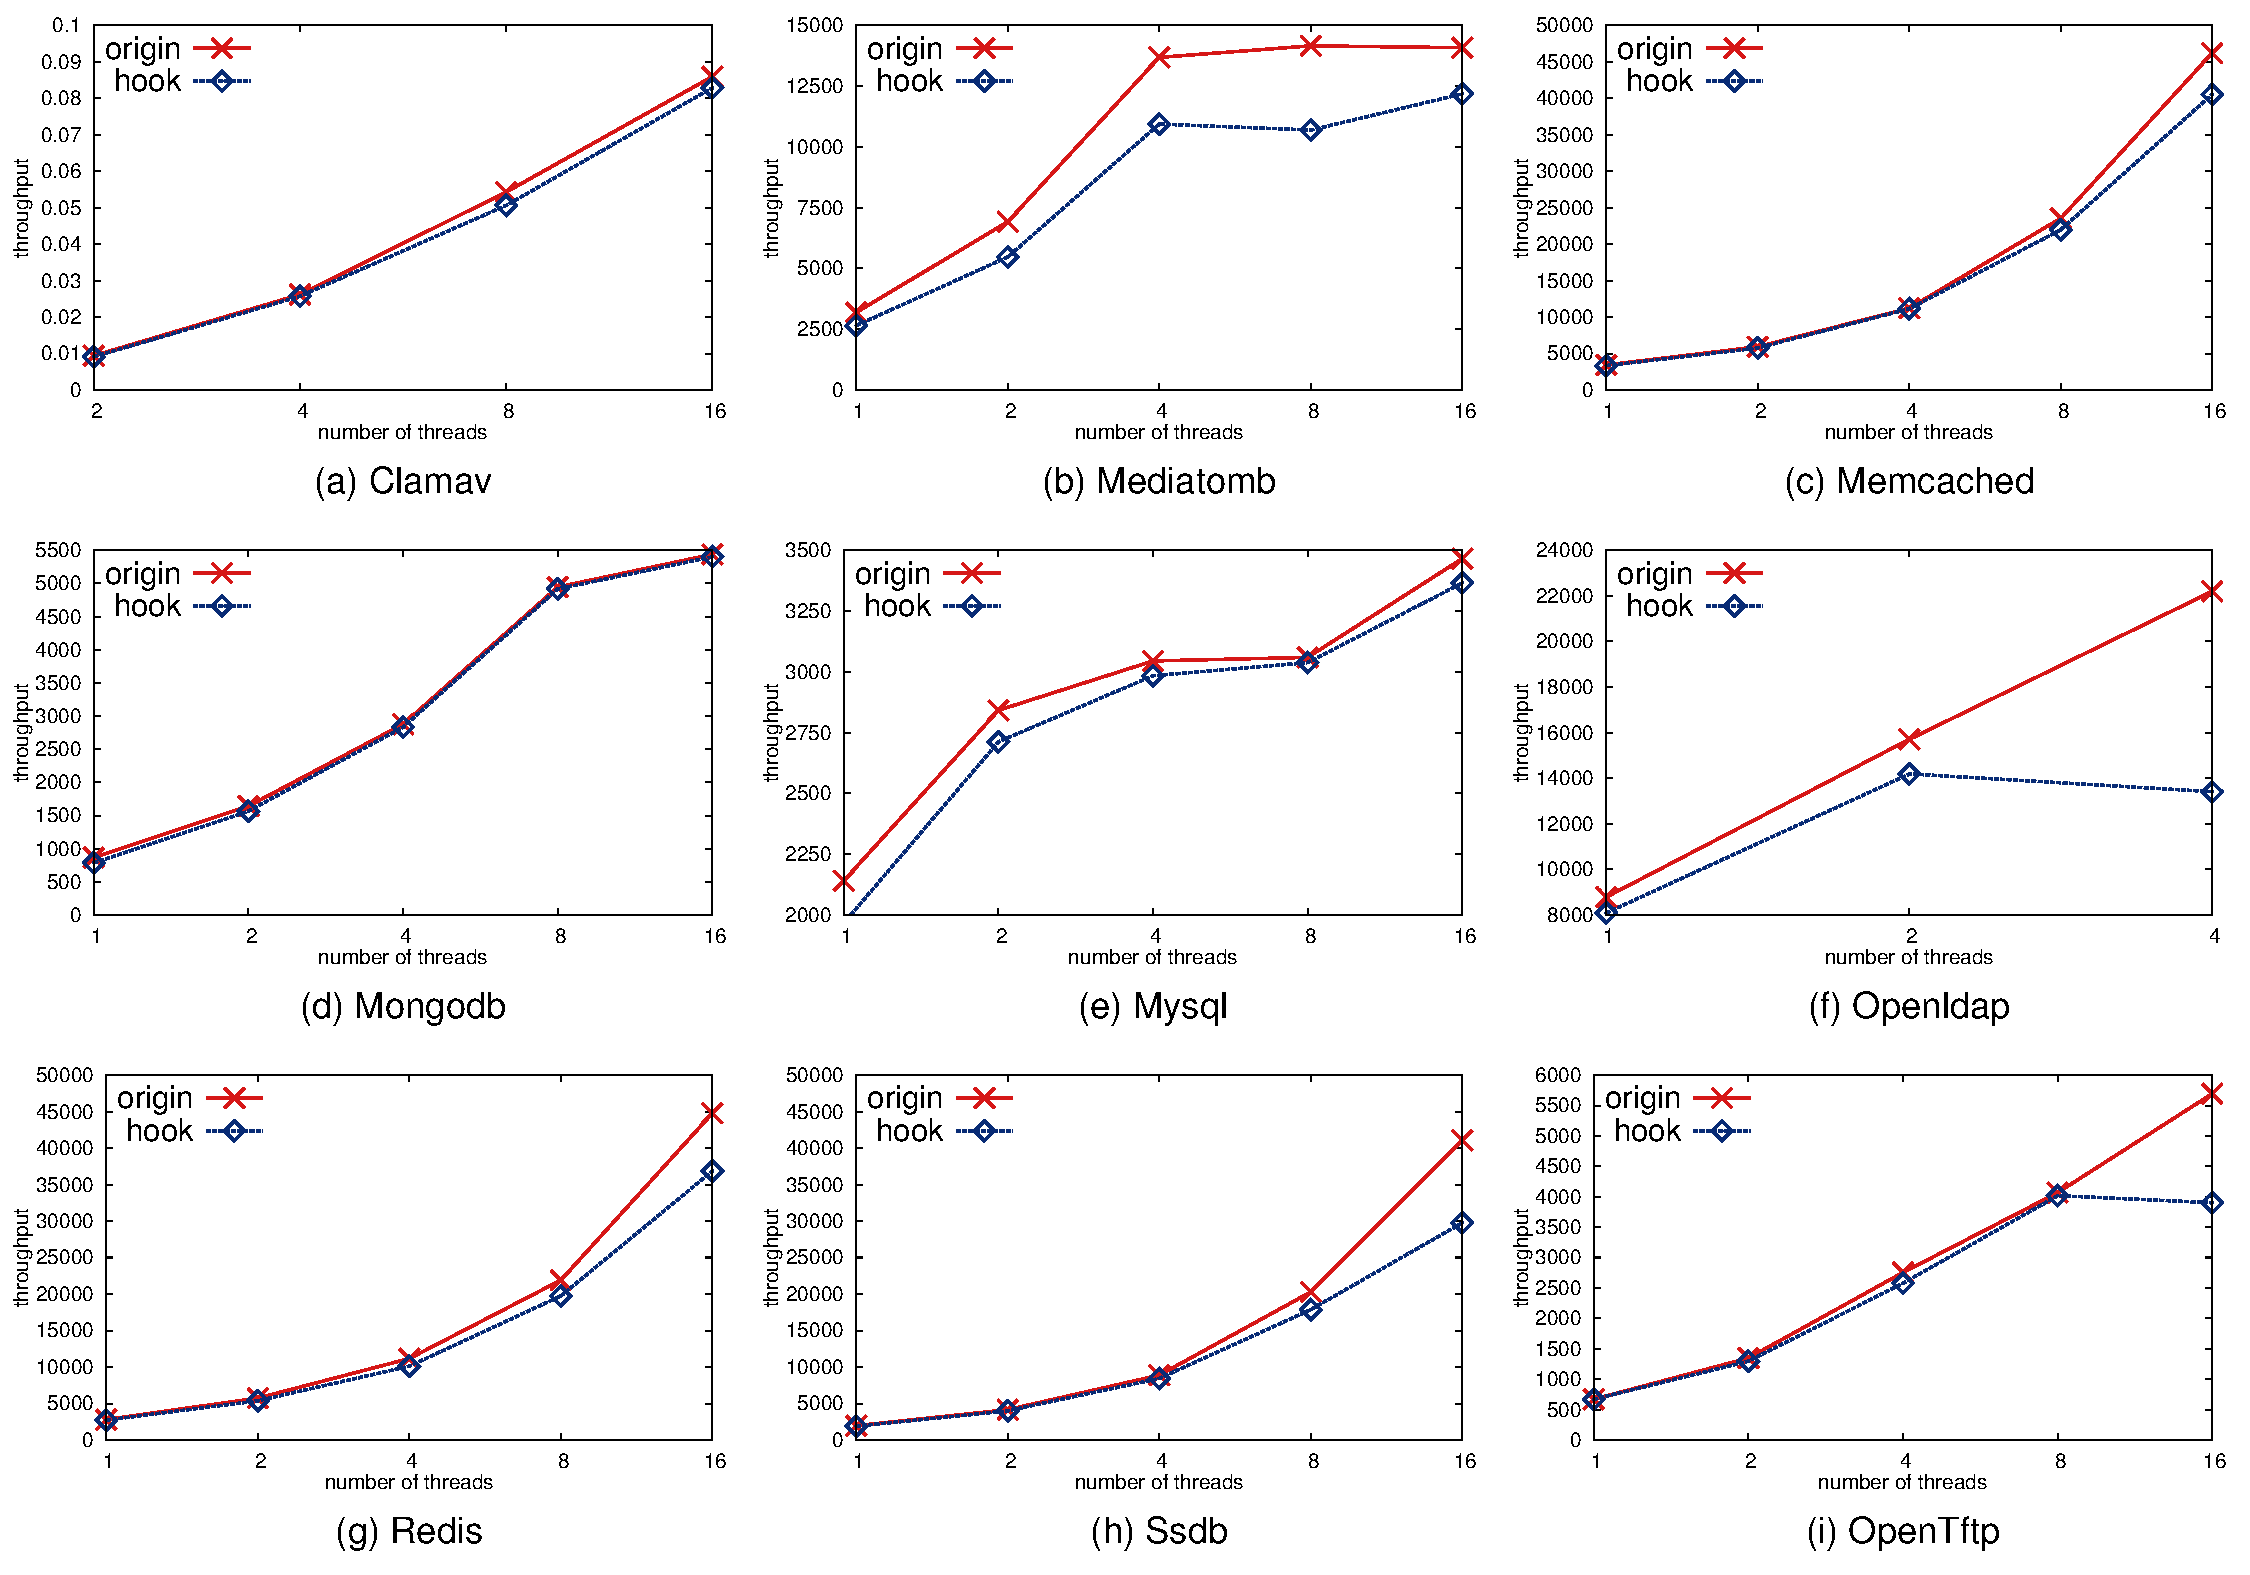
\includegraphics[width=0.9\textwidth]{figures/throughput}
\vspace{-.20in}
\caption{\small {\em \xxx throughput compared to the unreplicated 
execution.}}
\label{fig:tput}
\end{figure*}

\begin{figure}[t]
\centering
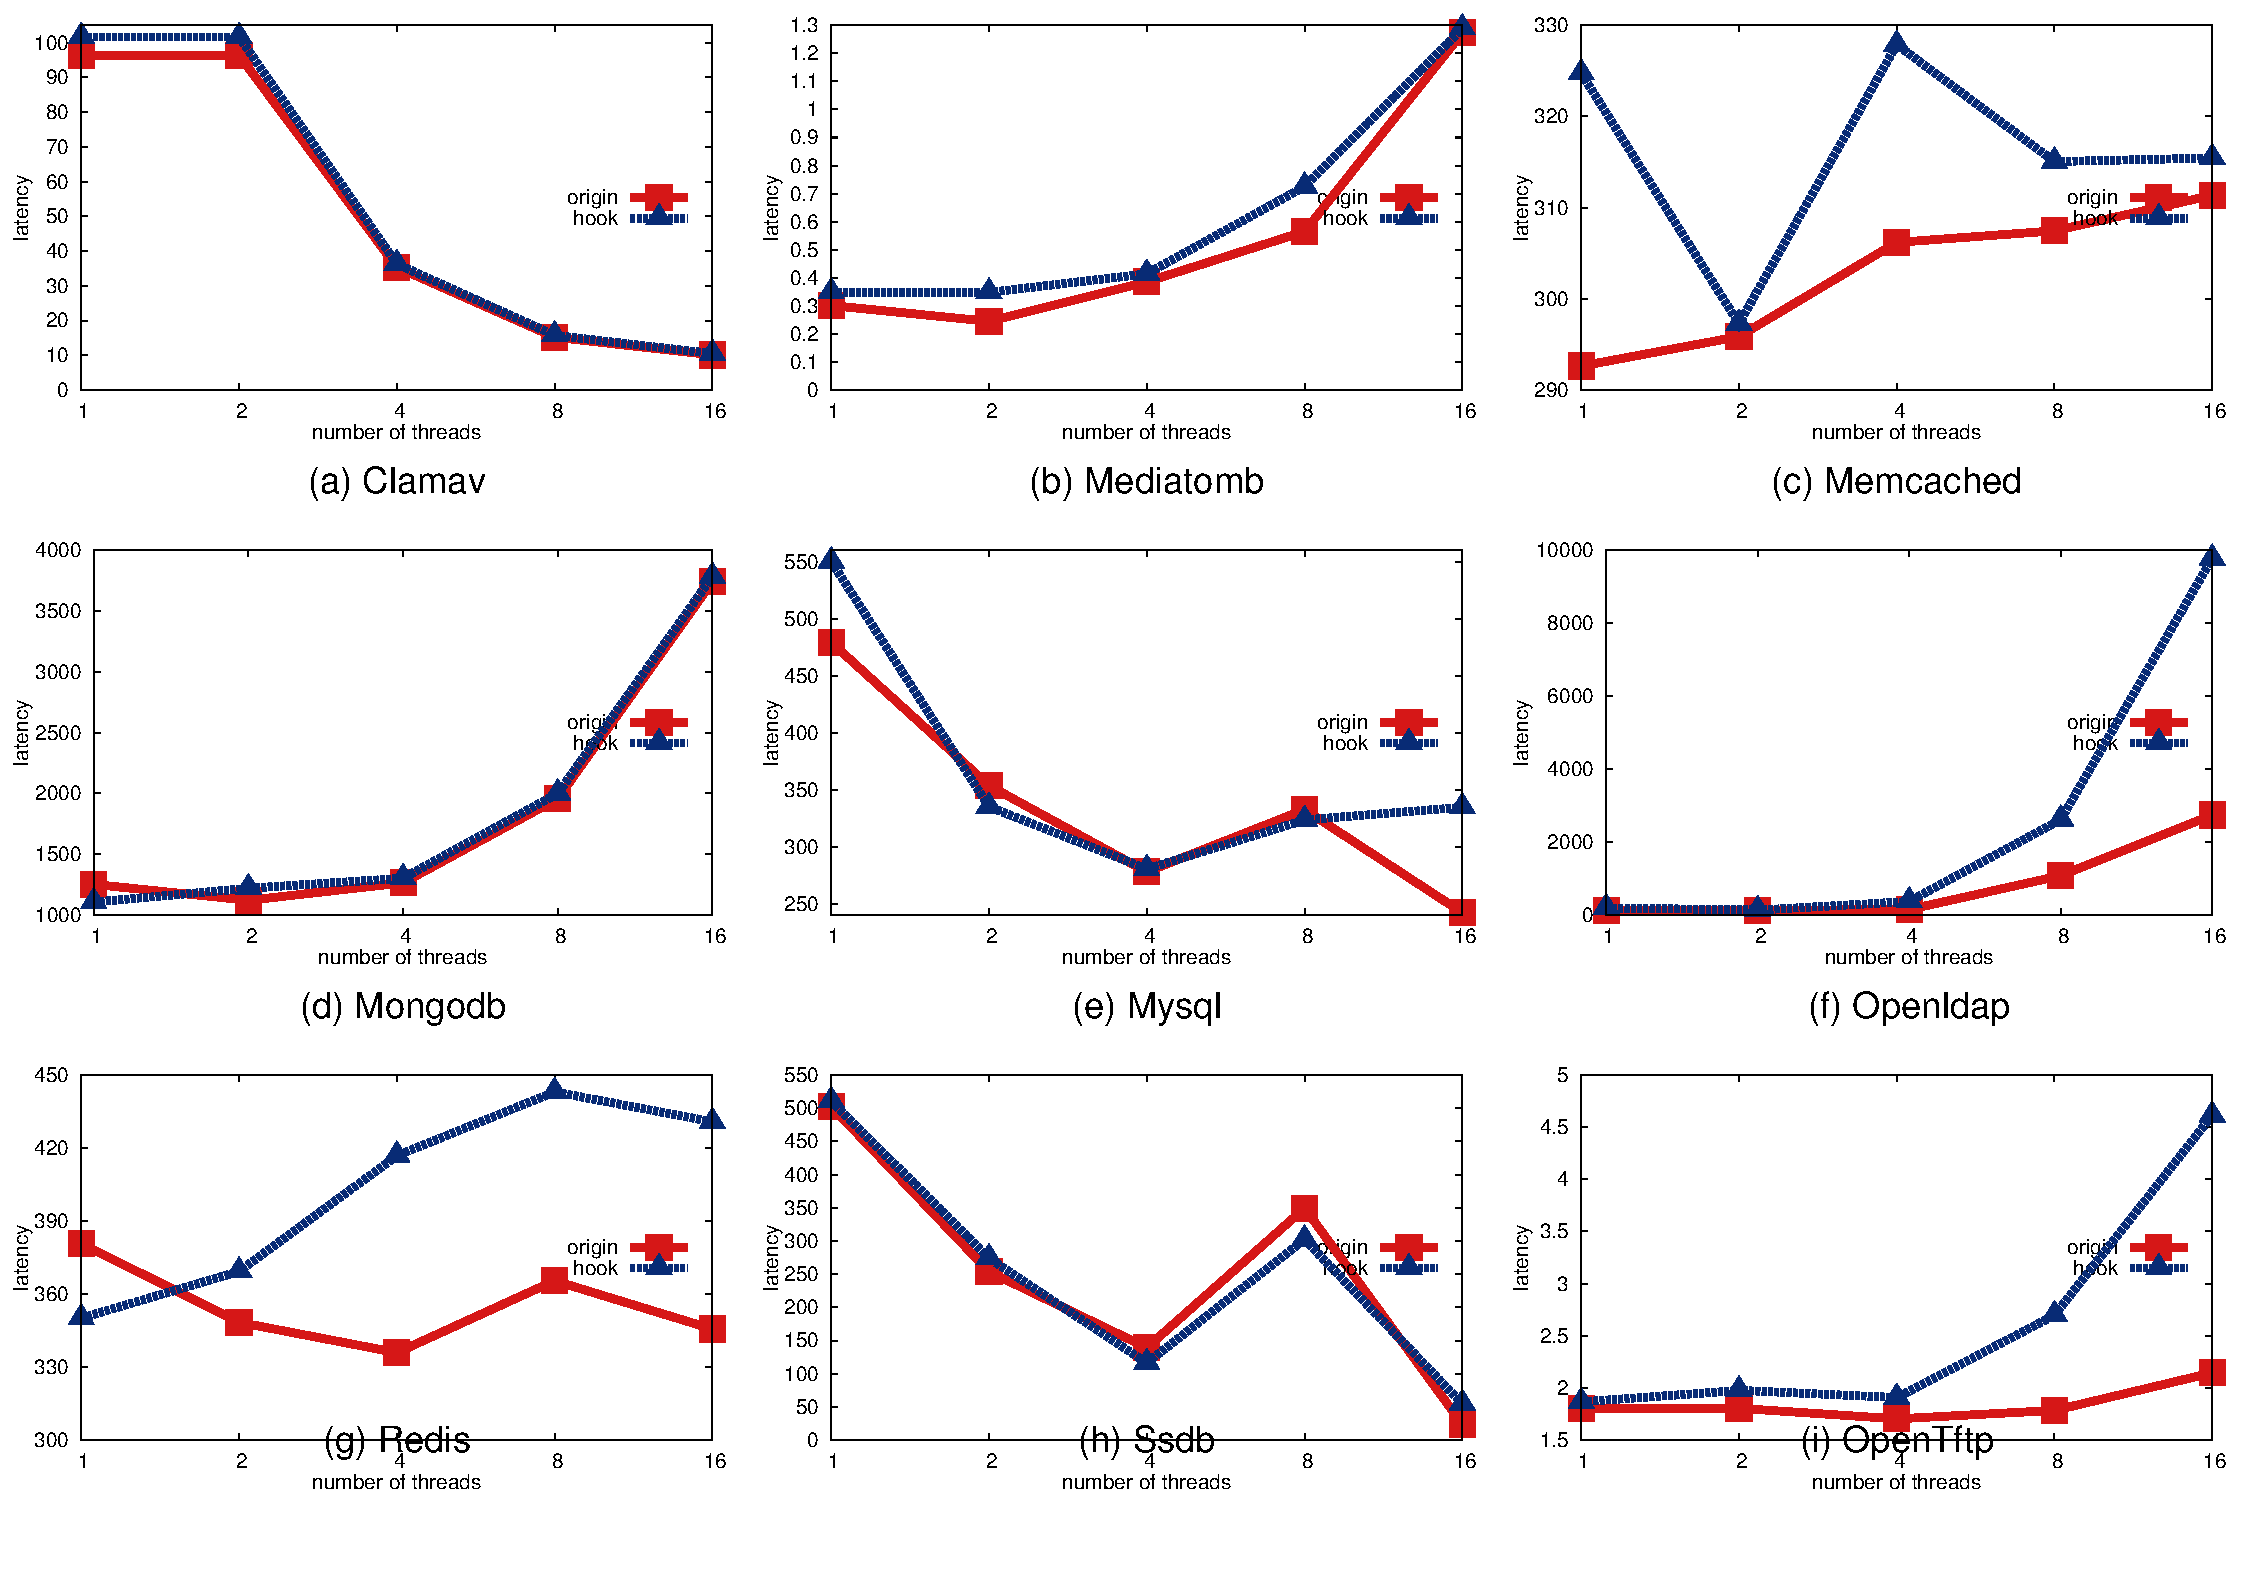
\includegraphics[width=0.9\textwidth]{figures/latency}
\vspace{-.20in}
\caption{\small {\em \xxx response time compared to the unreplicated 
execution.}}
\label{fig:latency}
\end{figure}

\begin{table}[b]
\footnotesize
\centering
\vspace{-.05in}
\begin{tabular}{lrrrrr}
{\bf Program} & {\bf \# calls} & {\bf input} & {\bf SSD} 
& {\bf quorum} & {\bf diff}\\
\hline\\[-2.3ex]
\clamav & 30  & 42.0 & 5.1 \us & 6.1 \us & F\\
\mediatomb & 3,000  & 140.0 & 4.7 \us & 5.8 \us & F?\\
\memcached & 10,016  & 38.0 & 4.9 \us & 6.9 \us & F?\\
\mongodb & 25,665  & 492.4 & 19.1 \us & 20.4 \us & F?\\
\mysql & 13,111  & 26.0 & 5.0 \us & 15.7 \us & W?\\
\openldap & 8,040  & 27.3 & 5.7 \us & 7.1 \us & T\\
\redis & 10,016  & 107.0 & 3.6 \us & 6.3 \us & T\\
\ssdb & 9,916  & 47.0 & 3.7 \us & 10.make cl9 \us & F*\\
\calvin & TBD  & TBD & TBD  & TBD & TBD\\
\end{tabular}
\vspace{-.05in}
\caption{{\em \xxx micro events.} The ``\# Calls" column means the number of 
socket calls that went through \xxx input concensus; ``input" means average 
bytes of a server's inputs received in these calls; ``SSD" means the average 
latency on storing these calls to stable storage; ``quorum" means the
average latency on waiting quorum for these calls; and ``diff" means whether 
the output checker found output divergence.} 
\label{tab:consensus-latency}
\end{table}


TBD.
% Overhead compared with unreplicated executions.

TBD.
% Bare consensus latency, micro events.

\subsection{Scalability on Replica Group Size} \label{sec:scalability}

TBD.
% 3, 5.

\subsection{Comparison with Traditional SMR systems} \label{sec:compare}

TBD.
% Run Calvin on Zookeeper, Crane, and Falcon. Because we can only make Calvin's 
% database with Zookeeper. XX speedup.

\subsection{Recovering from Output Divergence} \label{sec:robust}

TBD.
% Change 

\subsection{Sensitivity of Parameters} \label{sec:sensitivity}

% Change output comparison periods. 1, 100, 1000, 10000. 1000 is the smallest 
% number that starts to have negligible overhead. Run only with the server with 
% largest recv() data size.

% Twait

% Tcomphash
 
% \subsection{Read-only Optimization} \label{sec:read-opt}

% % 
\section{Related Work} \label{sec:related}


\para{Software-based consensus.} There are a rich set of
\paxos algorithms~\cite{paxos:practical,paxos,paxos:simple,paxos:complex,
epaxos:sosp13} and 
implementations~\cite{paxos:live,paxos:practical,chubby:osdi,crane:sosp15}. 
\paxos is notoriously difficult to be fast and 
scalable~\cite{ellis:thesis,manos:hotdep10,scatter:sosp11}. Since consensus 
protocols play a core role in datacenters~\cite{matei:hotcloud11, mesos:nsdi11, 
datacenter:os} and worldwide 
distributed systems~\cite{spanner:osdi12,mencius:osdi08}, a variety of study 
have been conducted to improve specific aspects of consensus protocols, 
including order commutativity~\cite{epaxos:sosp13}, 
understandability~\cite{raft:usenix14,paxos}, and verifiable reliability 
rules~\cite{modist:nsdi09,demeter:sosp11}.

% Although \xxx tightly integrates 
% RDMA features in \paxos, its implementation mostly complies with a popular, 
% practical approach~\cite{paxos:practical} for reliability. Other \paxos 
% approaches can also be leveraged in \xxx.


To make \paxos's throughput scalable (\ie, more replicas, higher throughput), 
various systems leverage \paxos as a core building block to develop advanced 
replication approaches, including partitioning program 
states~\cite{scatter:sosp11,dssmr,ssmr}, splitting consensus 
leadership~\cite{mencius:osdi08,spaxos}, and hieratical 
replication~\cite{manos:hotdep10,scatter:sosp11}. Theses approaches have shown 
to largely improve throughput. However, the core of these systems, 
\paxos, still faces an unscalable consensus 
latency~\cite{ellis:thesis,scatter:sosp11,manos:hotdep10}. By using \xxx as a 
building block, these system can scale even better.

% arious advanced replication models have been 
% developed~\cite{epaxos:sosp13,mencius:osdi08,scatter:sosp11,manos:hotdep10}. 



Three state machine replication (SMR) systems, Eve~\cite{eve:osdi12}, 
Rex~\cite{rex:eurosys14}, and Crane~\cite{crane:sosp15}, build traditional 
\paxos protocols to improve the availability of general server programs. 
Evaluation in these systems shows that SMR services incur modest overhead on 
server programs' throughput compared to their unreplicated executions. \xxx's 
consensus latency is one order of magnitude faster than traditional protocols 
(\S\ref{sec:eval-traditional}).
% If programs (\eg, key-value 
% stores) demand short request latency, \xxx  
% \xxx's (\S\ref{sec:compare}).
% These systems can leverage \xxx's general, 
% RDMA-accelerated protocol to improve latency.

% % DARE: simply use RDMA writes to do consensus on the leader side.
% To further improve consensus speed, DARE~\cite{dare:hpdc15} proposes a second 
% approach by simply replacing message passing in \paxos with one-sided RDMA 
% operations. For speed, DARE lets the leader handle a whole consensus round
% with three steps. The leader first appends a consensus request to a consensus 
% log in all remote replicas with RDMA writes. For the the successful writes with 
% ACKs, it then updates the tail pointers in remote logs and wait ACKs of these 
% updates. Finally, the leader knows that the minimum tail pointer among at 
% least a majority of replcias reach consensus.

% Two systems Rex and Eve did not provide latency evaluation; not open source.
% Two systems Calvin and Crane, we ran them with Calvin's database; we are XX 
% times faster.

% Notably, Eve~\cite{eve:osdi12} presents an execution state checking approach 
% based on their \paxos coordination service. Eve's completeness on detecting 
% execution divergence relies on whether developers have manually annotated all 
% thread-shared states in program code. \xxx's output checking approach is 
% automated (no manual code annotation is needed), and its completeness depends on 
% whether the diverged execution states propagate to network outputs. Eve and 
% \xxx's checking approaches are complementary and can be integrated.

% Two DARE limitations: first, no stable storage. second, old leader may 
% % unsafely writes to remote logs and thought it has reached a consensus.
% The second category includes DARE~\cite{dare:hpdc15}, a coordination protocol 
% that also uses RDMA to reduce latency. Part of \xxx's implementation was 
% inspired by DARE. \xxx differs from DARE in two major aspects.
% 
% The first difference is in a reliability model level. DARE's model is different 
% from standard \paxos's: DARE assumes that a replica's memory is still accessible 
% to remote replicas even if this replica's CPU fails, so that DARE's leader can 
% still write to remote backups. With this reliability model, DARE requires four 
% one-sided RDMA writes in each consensus round between the leader and a backup. 
% DARE's paper shows that the MTTF (mean time to failure) of memory and CPU are 
% similar.
% 
% \xxx's reliability model complies with standard \paxos's: memory 
% and CPU may fail, thus consensus requests must be written to stable storage. 
% \xxx requires two one-sided RDMA writes and two SSD writes on a consensus 
% round between the leader and a backup. DARE reported a $\sim$15 \us consensus 
% latency for write requests and $\sim$7 \us for read requests on a 64-byte 
% payload. \xxx's consensus latency is compatible with DARE's on a similar 
% payload size (\eg, \xxx's consensus latency for \ssdb was 14.6 \us in 
% Table~\ref{tab:consensus-latency}).

% Second, in a protocol level, DARE does pure-leader consensus in normal case 
% for efficiency. The leader writes a consensus request to remote replicas' 
% logs. If a majority of writes succeed with RDMA ACKs, the leader thinks that a 
% consensus has reached. DARE's backups do not invoke any proposal 
% number~\cite{paxos:simple} or view~\cite{paxos:practical} checking during 
% consensus.
% 
% In general, we argue that a pure-leader consensus approach is difficult to 
% guarantee safety. For instance, a leader may disconnect from the network 
% shortly (\eg, a temporary NIC error), reconnect, and then invoke 
% consensus requests. Concurrently, backups may start a leader election. It could 
% be risky that the leader's RDMA writes succeed and it ``thinks" that a 
% consensus has reached (because it handles everything of a consensus without any 
% backup involvement), but backups may have inconsistently started a leader 
% election.
% 
% Even if a backup first carefully does a check on a heartbeat timeout (or a 
% latest consensus request), it then closes the RDMA QP with this ``leader", 
% these two operations still have a vulnerable time window and the ``leader" can 
% write in between. Allowing a leader to ``think" that it has got a consensus 
% could be unsafe. This is probably why standard \paxos 
% protocols~\cite{paxos,paxos:simple,paxos:practical} must let backups do proposal 
% number of view checking rather than taking a pure-leader approach. \xxx complies 
% with standard \paxos protocol~\cite{paxos:practical}: a \xxx backup always 
% first compares its own view ID with the view ID in a consensus request, it then 
% agrees or rejects this request.

% The second difference is in an application level. DARE's evaluation used a 
% 335-line, single-threaded key-value store. \xxx aims to support general 
% programs.

% Various paxos protocols. Ours is complementary. Can be plugged into our 
% system.

% Three systems aim to provide SMR services to server programs. Eve, Rex, Dare, 
% Crane.
% Type I: Dare. Weaker durability. Four RDMA writes. We have two RDMA writes 
% plus two SSD writes. Compatible perf. Not for general server programs.

% Type II: Eve, Rex, Crane. All slow. Eve has output check, but also slow, use 
% TCP, and needs annotation.


\para{Hardware- or Network- assisted consensus.}  Three recent
systems~\cite{specpaxos:nsdi15,nopaxos:osdi16,hardware:paxos:nsdi16} leverage 
augmented network hardware or topology to improve \paxos consensus latency. 
``Consensus in a Box"~\cite{hardware:paxos:nsdi16} implemented \zookeeper's 
consensus protocol in FPGA and intensively modify its hardware TCP/IP stack for 
fast latency. It implemented a key-value store in hardware and showed similar 
consensus latency to \xxx on 3 or 5 replicas. It did not discuss or evaluate 
its scalability. Compared to this protocol, \xxx does not need to modify 
hardware, so it is easier to deploy and support general programs.

Speculative Paxos~\cite{specpaxos:nsdi15} and NOPaxos~\cite{nopaxos:osdi16} 
leverage the synchrony feature of datacenter topology to order requests, so 
they can eliminate consensus rounds if requests are not reordered or lost. 
Moreover, NOPaxos assigns a global sequence ID to requests so that it can 
proactively detect reordered or lost packets. If packets are lost or 
reordered, they invoke consensus to rescue. These two systems are not designed 
for scalability because when replica group becomes large, the probability that 
replicas incur ordered or lost requests may increase. Moreover, their consensus 
modules go through TCP/IP and have high round-trip latency, and \xxx can help.

\para{RDMA-based techniques.} RDMA techniques have been implemented in various 
architectures, including Infiniband~\cite{infiniband}, RoCE~\cite{roce}, and 
iWRAP~\cite{iwrap}. RDMA have been leveraged in many systems to improve 
application-specific latency and throughput, including high performance 
computing~\cite{openmpi}, key-value 
stores~\cite{pilaf:usenix14,herd:sigcomm14,farm:nsdi14,memcached:rdma}, 
transactional processing systems~\cite{drtm:sosp15,farm:sosp15}, and file 
systems~\cite{gibson:nfs}. These systems are largely complementary to \xxx. It 
will be interesting to investigate whether \xxx can improve the availability for 
both the client and server for some of these advanced systems within a 
datacenter, and we leave it for future work.

% \xxx's deployment model is to 
% provide SMR fault-tolerance to general server programs deployed in datacenters, 
% and the client programs access these server programs in LAN or WAN. 

% We didn't evaluate these systems because they are not available on client sides.


% Increasing assurance of replicas on thread schedulings. Not general 
% as Falcon's checkpoint techniques. But complementary for example ClamAV.
% \para{Nondeterminism.} 
% Nondeterminism~\cite{racepro:sosp11,dmp:asplos09,coredet:asplos10,
% cui:tern:osdi10, kendo:asplos09,
% dthreads:sosp11,peregrine:sosp11,parrot:sosp13,determinator:osdi10} is 
% pervasive in both application programs and OS kernels, and it often comes with 
% concurrency bugs~\cite{lu:concurrency-bugs}. To mitigate nondeterminism, 
% deterministic multithreading techniques~\cite{grace:oopsla09, 
% dthreads:sosp11, 
% determinator:osdi10,dpj:oopsla09, 
% dmp:asplos09,kendo:asplos09,coredet:asplos10,dos:osdi10,ddos:asplos13,
% ics:oopsla13} and deterministic replay 
% techniques~\cite{r2:osdi,friday2007,srinivasan:flashback,revirt,dejavu,
% vmware-record-replay,smp-revirt:vee08,pres:sosp09,scribe:sigmetrics10,
% odr:sosp09, capo:asplos09} have been developed. Much of these techniques can 
% greatly improve software reliability, but they often come with a performance 
% slowdown. \xxx can run these techniques with the server program to mitigate 
% replica divergence caused by concurrency bugs. 

% \para{Concurrency.} Pervasive in real-world applications. Threads. Processes. 
% Break SMR's state machine assumption. complementary.
% \para{Concurrency.} \xxx are mutually beneficial with much prior work on 
% concurrency error 
% detection~\cite{yu:racetrack:sosp,savage:eraser,racerx:sosp03,lu:muvi:sosp,
% avio:asplos06,conmem:asplos10},
% diagnosis~\cite{racefuzzer:pldi08,ctrigger:asplos09,atomfuzzer:fse08}, and
% correction~\cite{dimmunix:osdi08,gadara:osdi08,wu:loom:osdi10,cfix:osdi12}. 
% On one hand, these techniques can be deployed in \xxx's backups and help 
% \xxx detect data races. On the other hand, \xxx's asynchronous replication 
% architecture can mitigate the performance overhead of these powerful 
% analyses~\cite{repframe:apsys15}.



\section{Conclusion}\label{sec:conclusion}

We have presented \xxx, a fast, general state machine replication system 
through building an RDMA-accelerated \paxos protocol to efficiently coordinate 
replica inputs. On top of this protocol, \xxx introduces an automated, 
efficient output checking protocol to detect and recover execution divergence 
among replicas and improve the assurance of sync in replicas. Evaluation on 
widely used, diverse server programs shows that \xxx supports these unmodified 
programs with reasonable performance overhead, and can recover from replica 
divergence caused by real-world software bugs. \xxx has the potential to 
greatly increase the adoption of state machine replication and improve the 
reliability of general programs.

\end{sloppypar}

% uncomment to tweak with bib spacing
%\setlength\bibsep{2.25pt}
{
%\small
 \bibliographystyle{abbrv}
 \bibliography{bib/biblio}
}

\end{document}
